\chapter{Fretha的设计和开发}

\section{引言}

\ifshowtext
在现代生物医学研究中,FRET双杂交分析作为一种关键技术,用于检测生物分子间的相互作用,为揭示生物过程的分子机制提供了重要手段。
然而,传统的 FRET 双杂交分析数据处理过程繁琐且效率低下,严重依赖人工操作,容易引入误差。
开发专门针对 FRET 双杂交分析数据处理的配套软件,能够实现数据的自动化采集、标准化处理以及高效的分析统计,对于提升研究效率和准确性具有重要意义。
本章节首先根据我们组自研的用于高通量药物筛选的 FRET 显微成像系统(FRETscopeII)的硬件参数和 FRET 数据处理及 FRET 双杂交分析数据处理功能进行深入的需求分析。基于此需求分析,对软件按照功能进行科学合理的模块划分和总体框架设计。
接着,详细介绍软件的开发技术选型以及每个模块的具体实现方式,旨在全面展示 Fretha 软件从设计构思到开发实现的全过程。
\fi

\section{需求分析和总体设计}

\subsection{需求分析}

\ifshowtext
FRETscopeII是本课题组自研的适用于$3^3$-FRET、E-FRET、Pb-FRET等多种定量FRET分析方法的FRET多模态显微成像系统。该系统具备高分辨率成像、多通道同步采集等先进特性,能够获取高质量的 FRET 三通道图像数据。

% FRET双杂交分析数据处理流程。
使用FRETscopeII对制备好的样本进行图像采集得到若干视野的FRET三通道图像后,通过FRET双杂交分析方法定量计算细胞中的生物大分子结合作用的FRET饱和效率、化学计量比、相对亲和力等信息。FRET双杂交分析的数据处理需要如下步骤:首先需要对FRET数据进行数据完整性校验,确保每个视野下存在完整的三通道图像和文件完整可读,然后对每个视野进行荧光信号提取,通过在图像上绘制ROI并计算其灰度均值作为FRET分析计算重要的荧光信号;根据E-FRET和$3^3$-FRET方法将上述荧光信号代入对应的计算公式求取$E_A$、$E_D$、$R_C$等FRET数据;对这些数据进一步依据物理含义或者数据分析进行异常值去除等数据预处理;最后是通过优化算法拟合Langmiur模型或者线性模型计算相关的参数。具体流程如图 \ref{fig:tha_data_process} 所示。

\begin{figure}[hbtp]
    \centering
    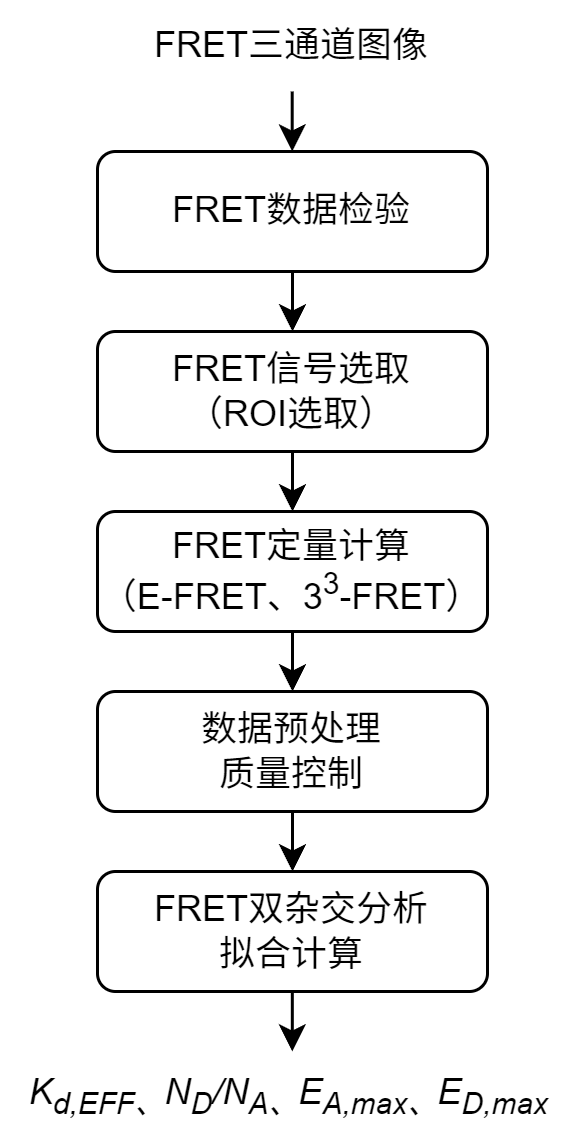
\includegraphics[width=0.4\linewidth]{../figures/2/2_FRET双杂交分析数据处理流程.png}
    \caption{FRET双杂交分析数据处理流程}
    \label{fig:tha_data_process}
\end{figure}

\fi

\subsection{模块划分和界面设计}

结合 FRET 双杂交分析的数据处理流程与功能逻辑,Fretha 软件主要划分为以下核心模块:

\begin{enumerate}
  \item \textbf{成像参数设置模块:}负责设置 FRET 成像过程中的关键参数,确保成像数据的准确性和一致性。
  该模块允许用户输入和保存成像参数,如曝光时间、光学参数等,并提供参数校验功能,确保输入的参数在合理范围内,避免因参数设置错误导致的数据分析问题。
  成像参数一般比较稳定,通常2到3个月才需要重新测量,因此需要持久化到本地,以供多次处理数据时使用。
  \item \textbf{数据检验模块:}对输入数据进行严格的完整性和合法性检验,避免异常数据导致的分析错误。
  该模块会检查每个视野的三通道图像文件是否完整,并对文件格式和内容进行验证,确保数据的可靠性。
  通过数据完备性检验,可以避免异常数据导致的分析错误,提高数据处理的准确性。
  \item \textbf{FRET 图像处理模块:}支持手动图像处理和 ROI 选取,满足用户对数据的精细化处理需求。
  用户可以在图像上手动圈选感兴趣区域(ROI),并进行图像增强、滤波等处理操作。
  该模块提供多种图像处理工具,帮助用户提高图像质量和分析精度。
  手动选取感兴趣区域ROI是一个基础且关键的操作,它能帮助分析人员聚焦于细胞中荧光质量较高的区域,进行更精确的数据处理与分析。
  结合LURS(Luminance-Uniformity-based ROI Selection)算法实现自动 ROI 选取,减少人工操作,提高处理速度和一致性。
  \item \textbf{数据管理模块:}
  数据处理模块用于增删数据、筛选数据、导入导出、开始计算等功能,还可以根据记录表中的数据项在FRET图像处理模块定位所选数据的ROI。
  \item \textbf{结果可视化模块:}将分析结果以直观的图表形式展示,并提供数据保存功能,方便用户进一步分析和应用。
  该模块支持多种图表类型,如趋势线图、散点图等,用户可以根据需要选择合适的图表进行数据展示和分析。
  通过结果可视化,用户可以更直观地理解分析结果,比如分析FRET双杂交分析结果的相关性、拟合程度等,从而确保数据处理的准确性和可靠性。
  结果可视化模块还可以将分析结果保存为图片或数据文件,方便用户进行后续数据处理和报告撰写。
  
\end{enumerate}

在界面设计上,根据软件使用需求和模块功能,主要分为:开始页、参数设置页、数据处理页、结果页。
在软件开始页提供了跳转参数设置页或数据处理页的按钮,如图 \ref{fig:开始页界面} 所示;
\begin{figure}[hbtp]
  \centering
  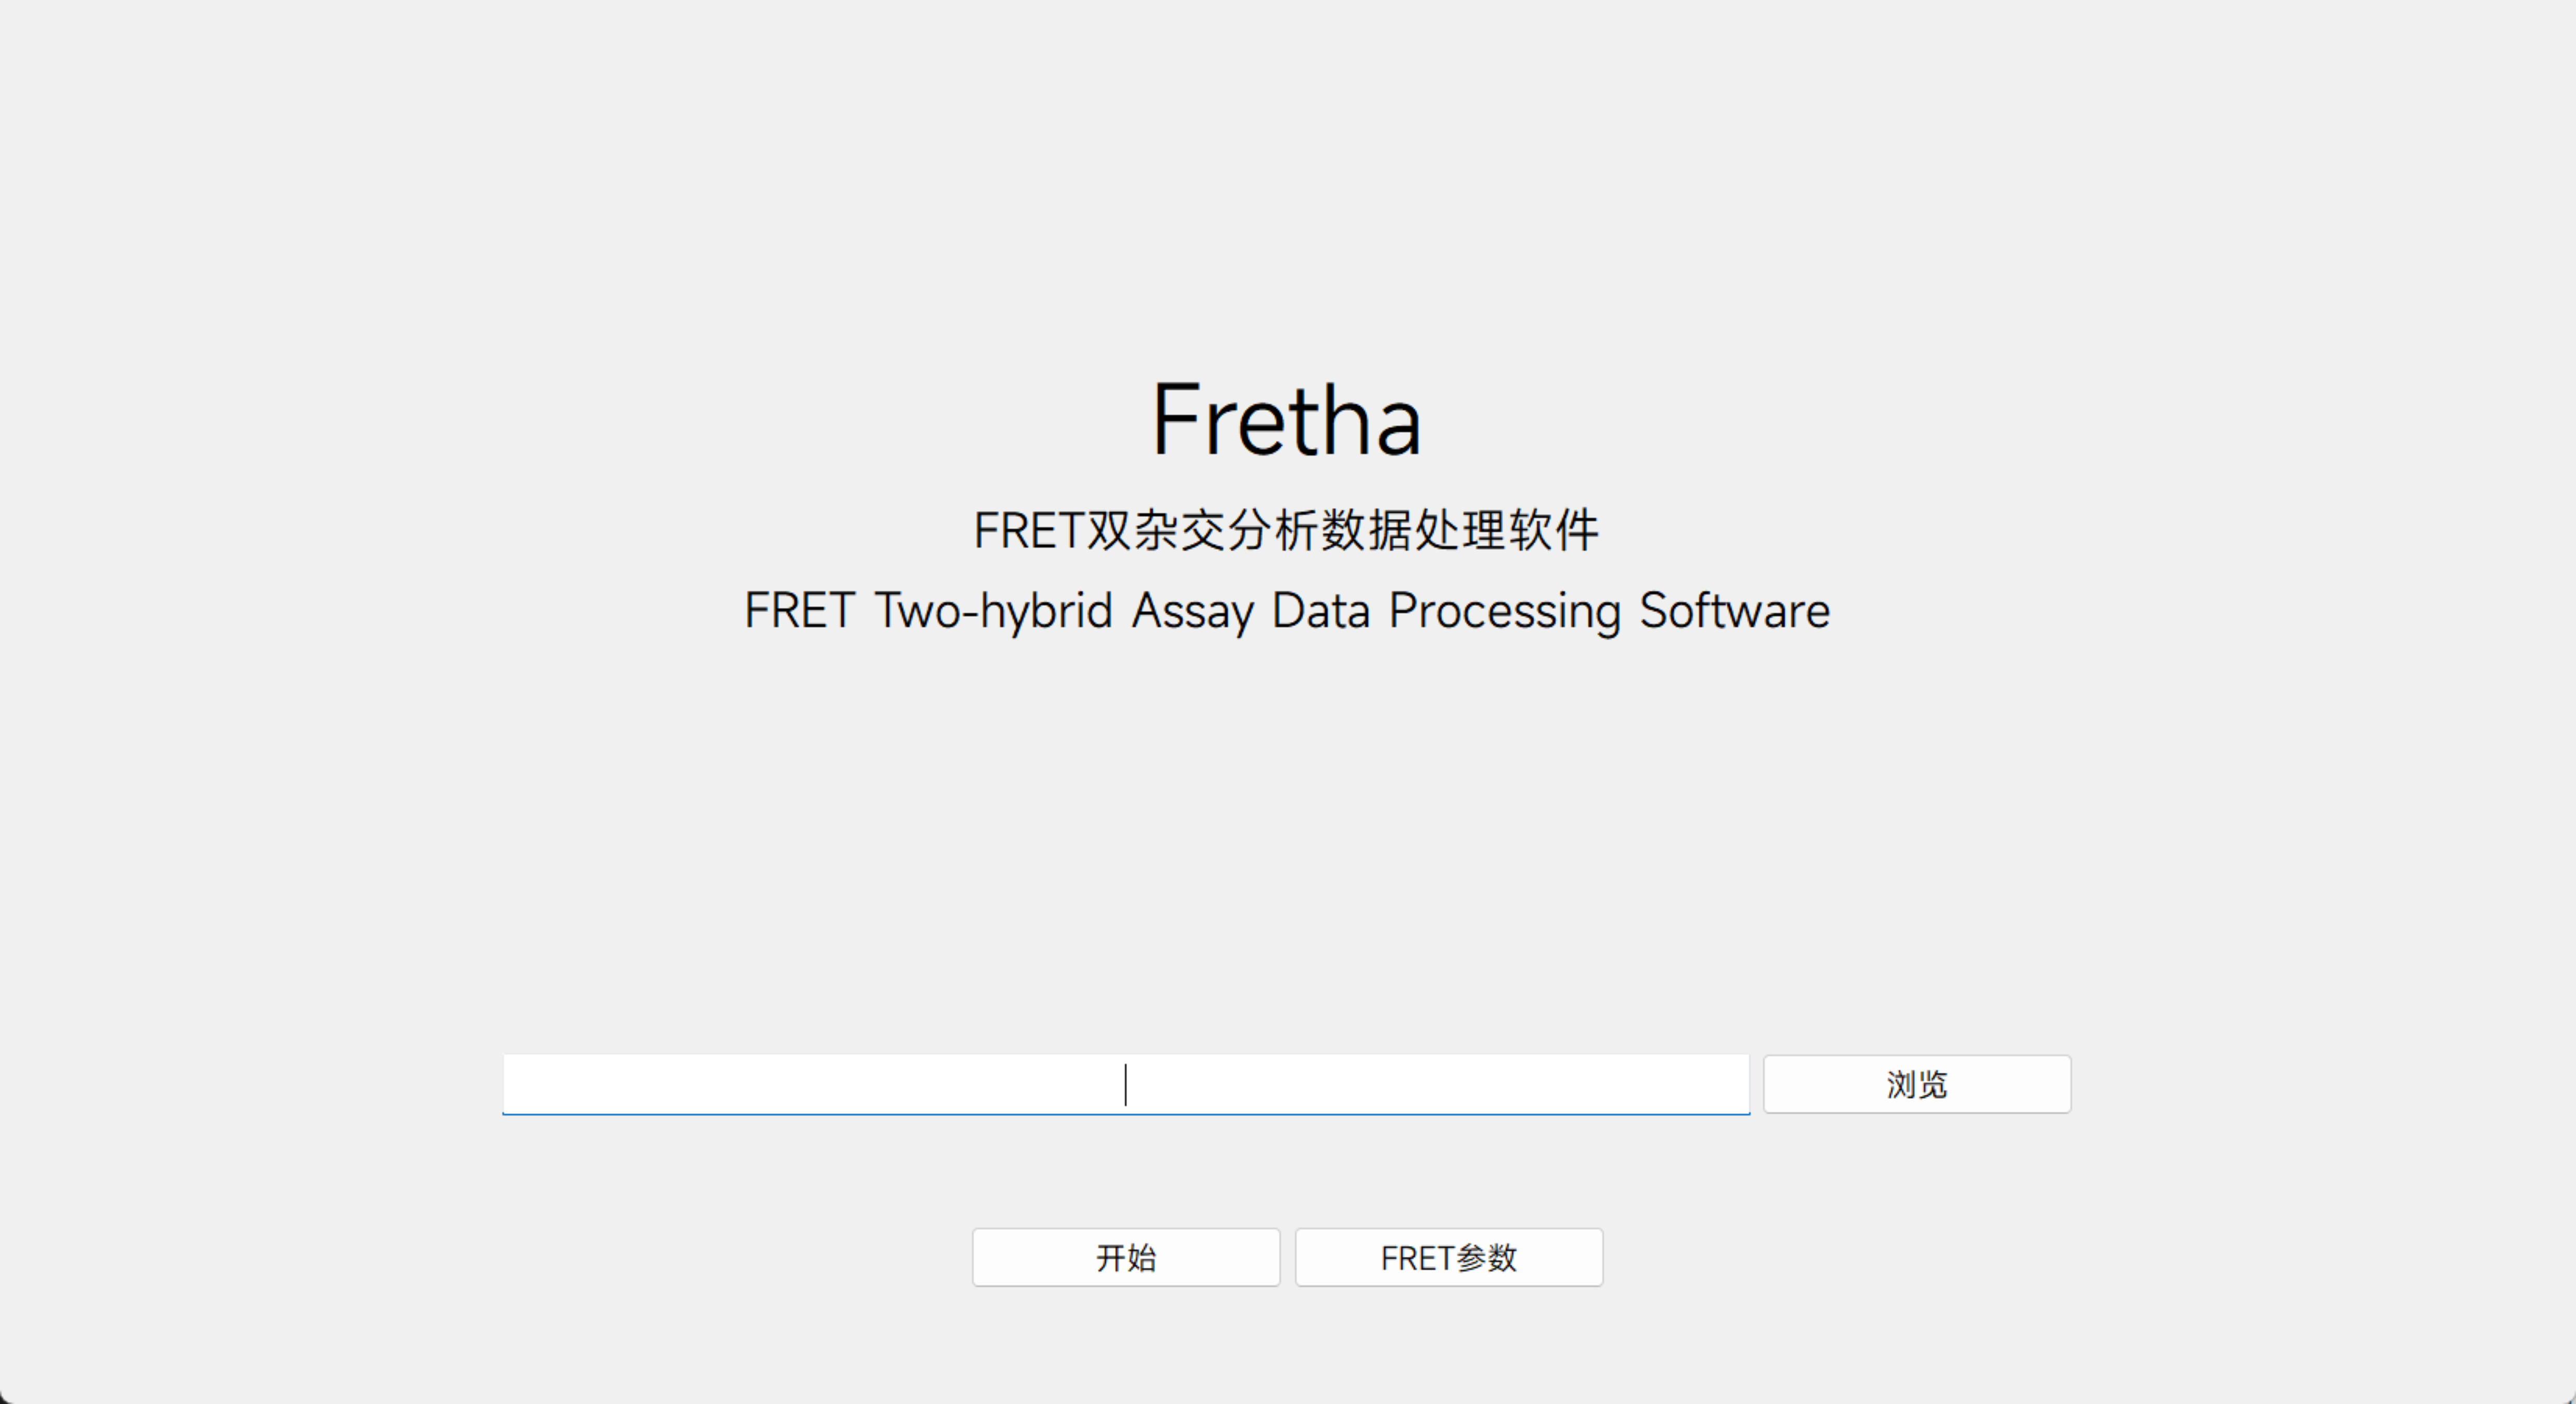
\includegraphics[width=0.9\linewidth]{../figures/2/2_开始页界面.png}
  \caption{Fretha开始页界面}
  \label{fig:开始页界面}
\end{figure}
参数设置页面包括成像参数设置模块,其界面如图 \ref{fig:参数设置页界面} 所示;
\begin{figure}[hbtp]
  \centering
  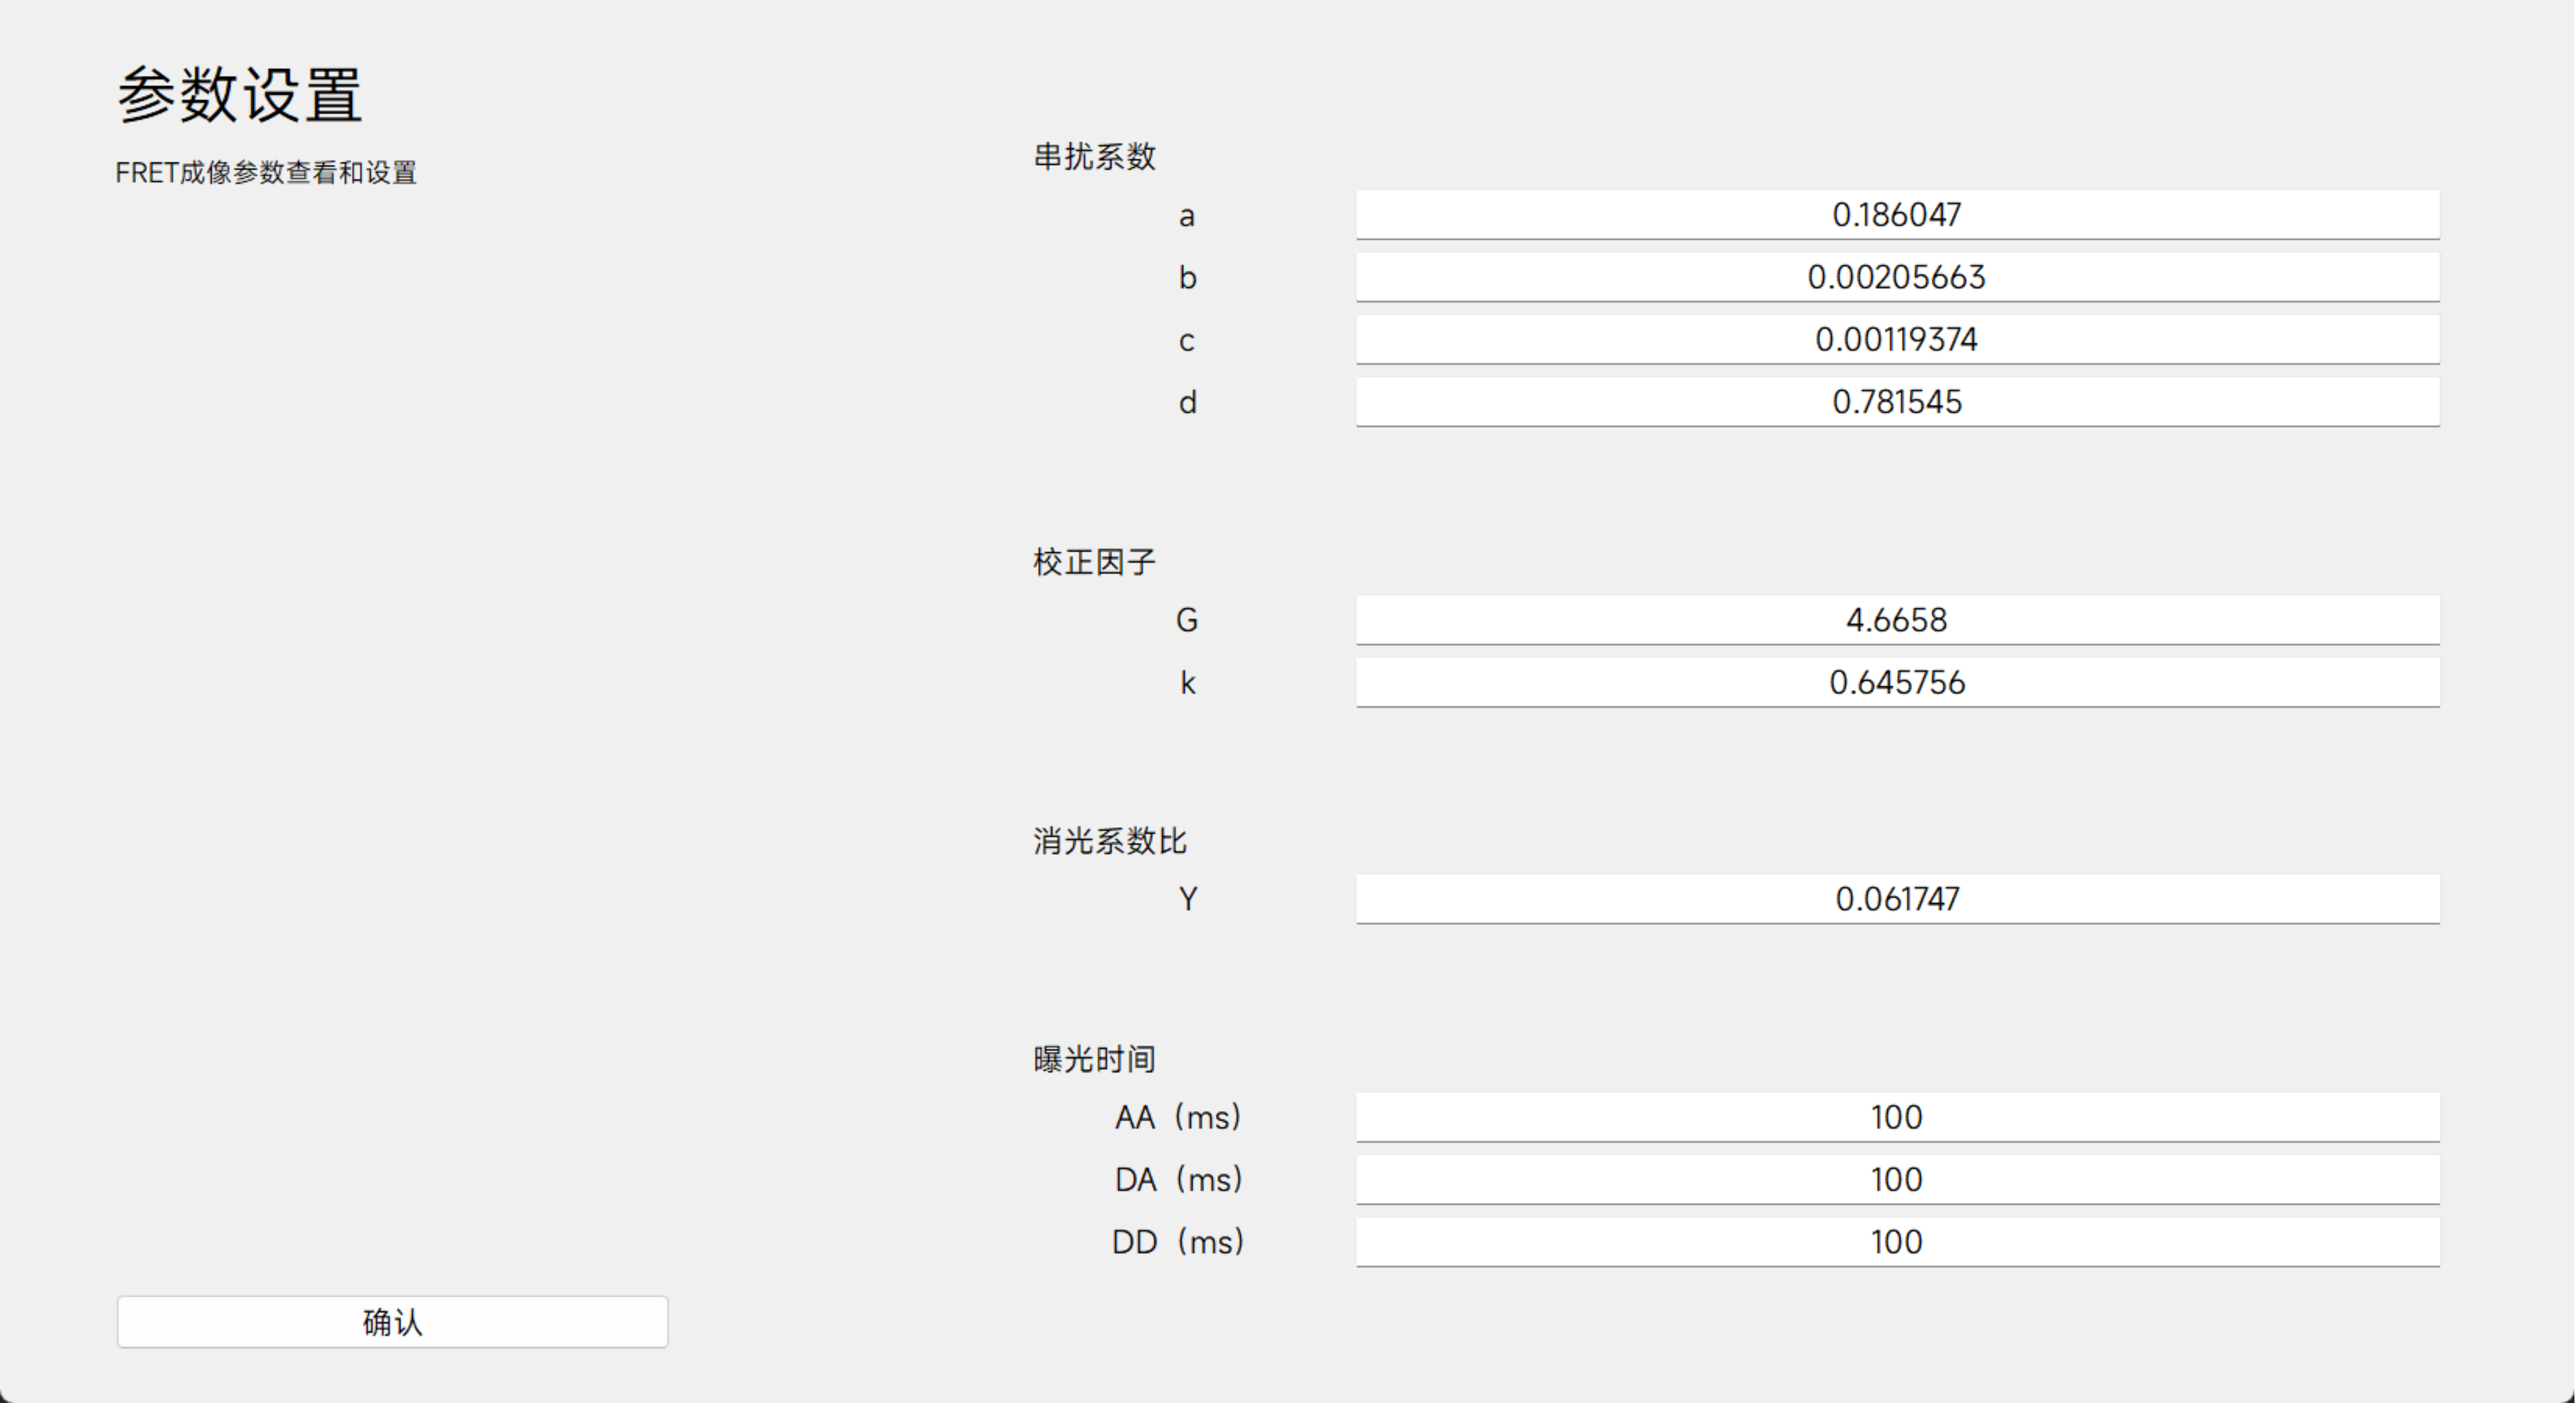
\includegraphics[width=0.9\linewidth]{../figures/2/2_参数设置界面.png}
  \caption{Fretha参数设置页界面}
  \label{fig:参数设置页界面}
\end{figure}
数据处理页包括数据检验模块的检验结果、FRET图像处理模块、数据管理模块,其界面和模块划分如图 \ref {fig:界面模块分布图} 所示;
\begin{figure}[hbtp]
  \centering
  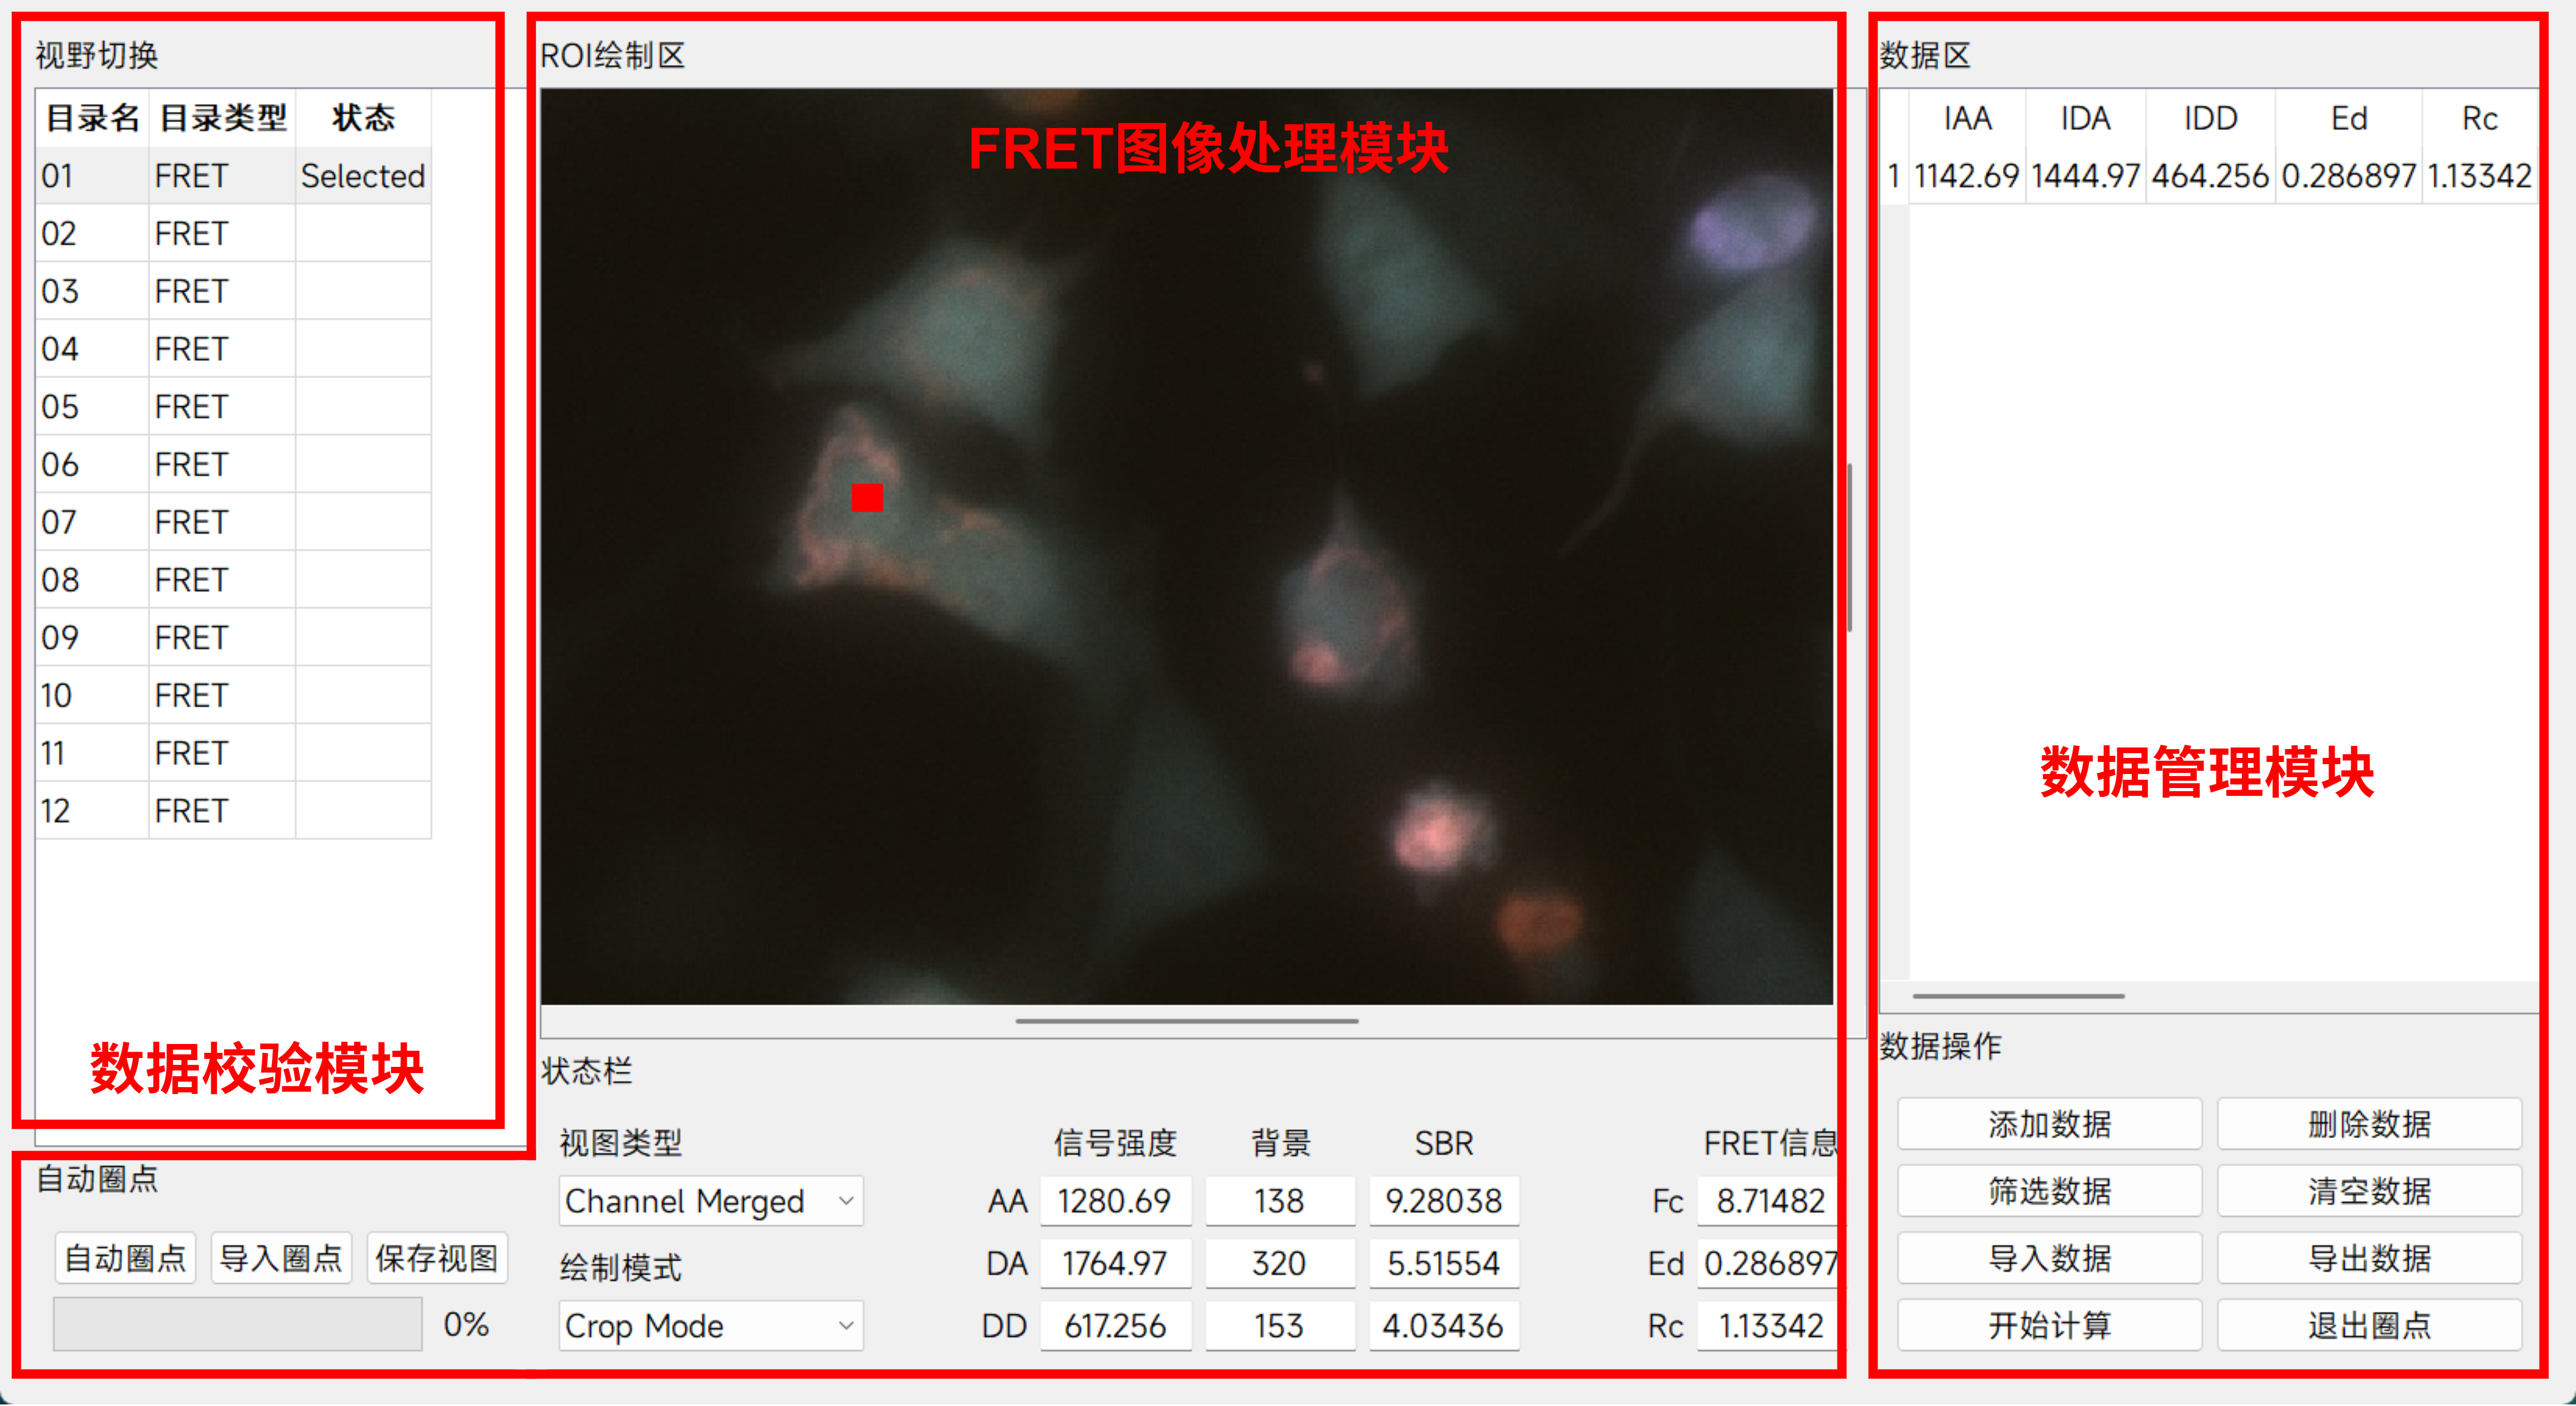
\includegraphics[width=0.9\linewidth]{../figures/2/2_模块界面.png}
  \caption{Fretha数据处理页界面及模块划分}
  \label{fig:界面模块分布图}
\end{figure}
结果页展示结果可视化模块中FRET双杂交数据处理的图像视图结果,界面如图 \ref{fig:fretha_result_ui} 所示。
\begin{figure}[hbtp]
  \centering
  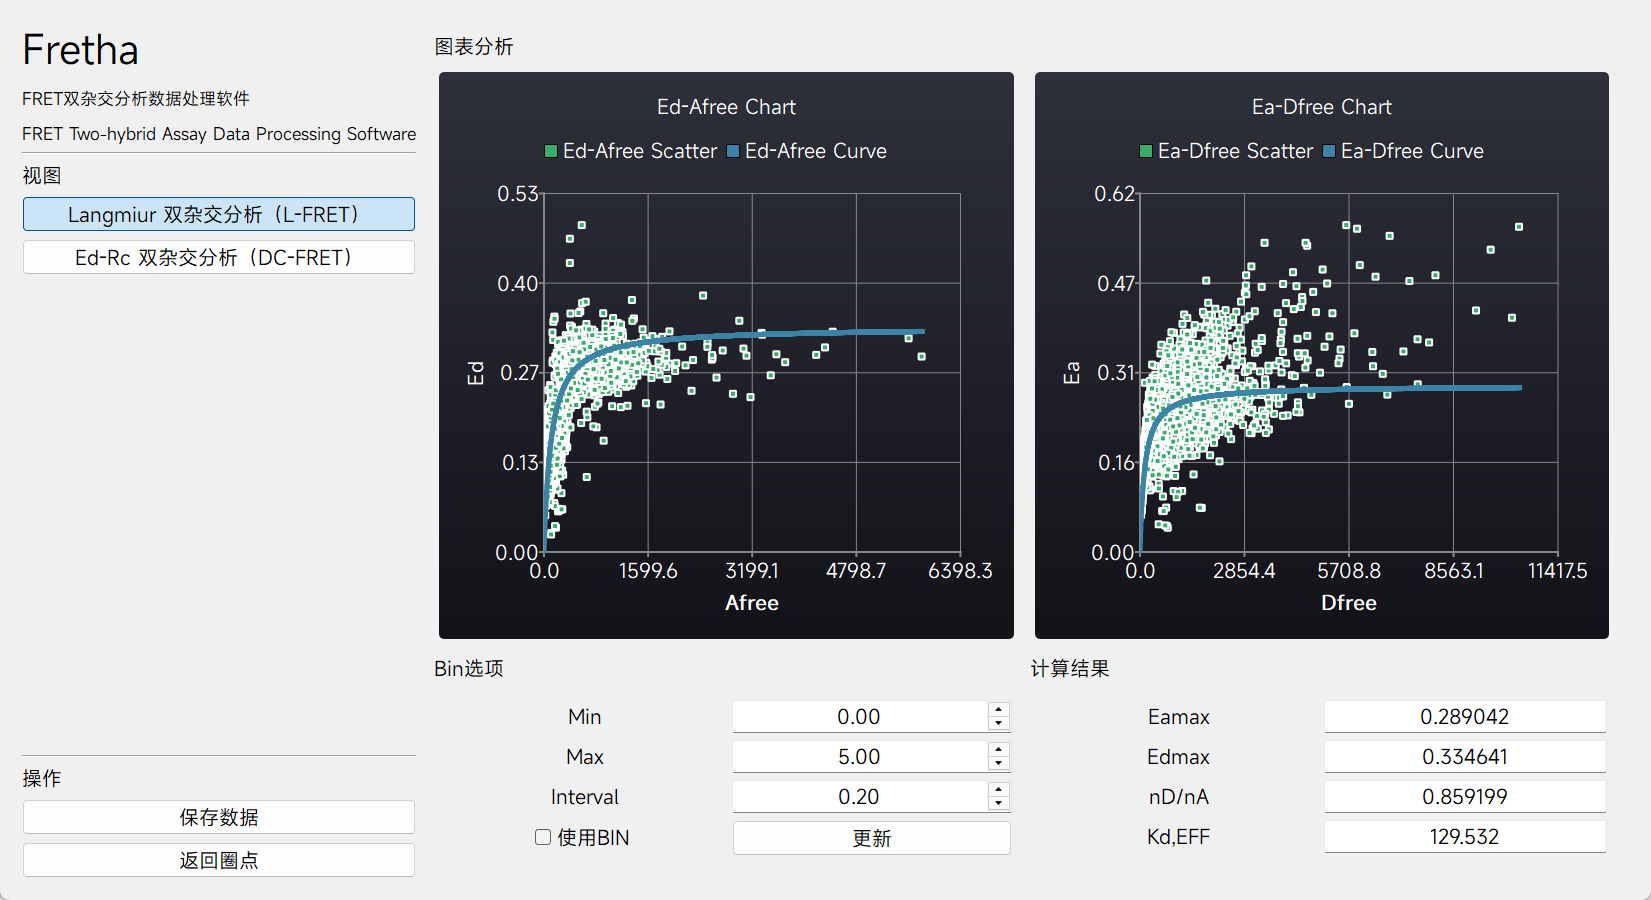
\includegraphics[width=0.9\linewidth]{../figures/2/2_结果可视化.png}
  \caption{Fretha结果可视化模块界面}
  \label{fig:fretha_result_ui}
\end{figure}

\subsection{软件总体框架}

Fretha架构采用分层设计,由顶层向下依次分别为:表现层、业务层、数据访问层和数据层,如图 \ref{fig:fretha_arch} 所示。

\begin{figure}[hbtp]
    \centering
    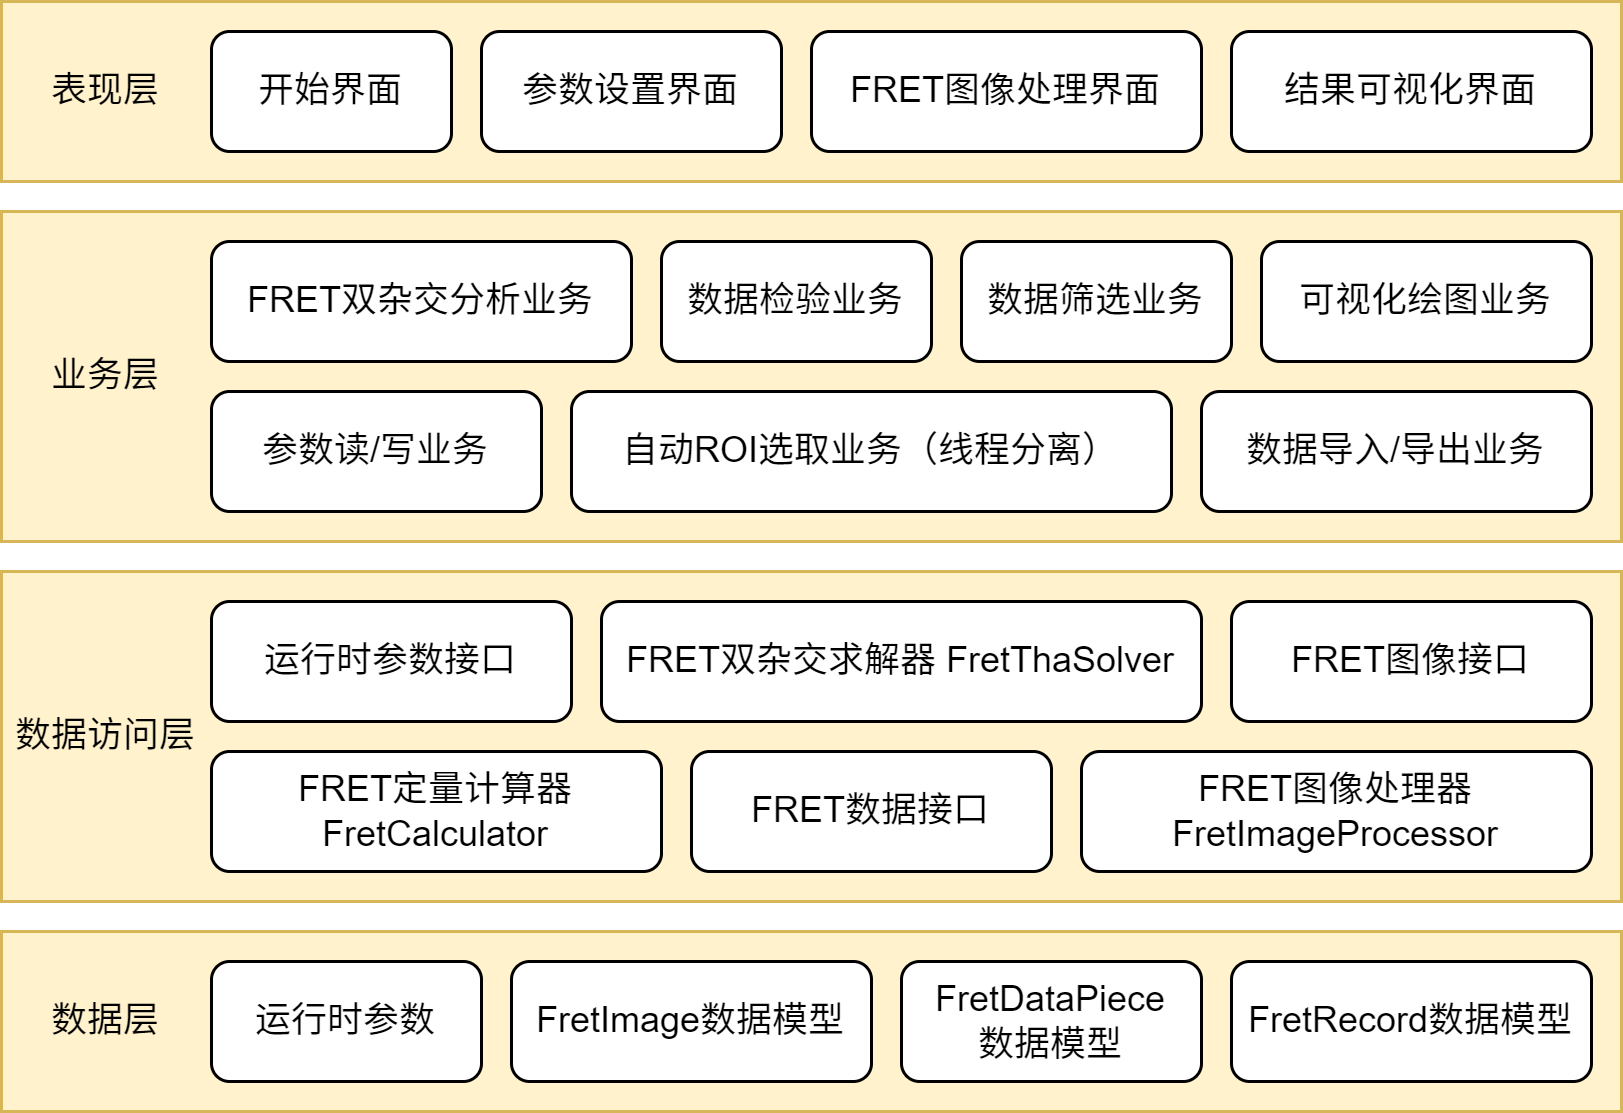
\includegraphics[width=0.9\linewidth]{../figures/2/2_Fretha架构.png}
    \caption{Fretha软件总体架构}
    \label{fig:fretha_arch}
\end{figure}

表现层(Presentation Layer)处于整个架构的最外层,直接面向用户,是用户与系统进行交互的主要界面。
它负责接收用户输入的各种指令和数据,并以直观、友好的方式展示系统的处理结果。
Fretha的表现层主要包括开始界面、参数设置界面、FRET图像处理界面、结果可视化界面等,用户能够通过表现层的软件界面与系统进行交互,完成FRET双杂交分析的数据处理操作。

业务层(Business Logic Layer)是整个架构的核心逻辑处理部分,承担着对系统业务规则和流程的实现。
它接收来自表现层的请求,根据预设的业务逻辑对数据进行处理和转换。
Fretha的业务层封装了包括参数读/写业务、数据检验业务、自动ROI选取业务、数据导入/导出业务、FRET双杂交分析业务、可视化绘图业务等。

数据访问层(Data Access Layer)实现对数据的访问和操作,它将业务层与数据层进行隔离。
数据访问层提供了统一的数据访问接口,业务层通过调用这些接口来获取和存储数据,而无需关心数据的具体存储方式和位置。
通过设置数据访问层,能够使得在复杂的业务处理时避免对数据的直接操作和影响,从而提高了数据存储的安全性。
Fretha的数据访问包括FRET图像数据访问、FRET数值数据访问和FRET双杂交数据访问的接口。
特别地,在数据访问层还包括FRET定量计算器和FRET图像处理器、FRET双杂交求解器等,它们除了可以作为数据访问层的接口,还可以完成FRET计算分析作为业务层的业务逻辑处理单元,这样的设计减少了业务层设计的复杂度,提高了系统的可维护性和可扩展性。

最后是数据层(Data Layer),作为架构的最底层,数据层负责存储系统的所有数据。
Fretha数据层包括系统静态数据、FretImage类、FretDataPiece类和FretRecord类。
系统静态数据是在软件运行时的环境参数,只需要在指定步骤运行前提前设置好即可,如成像参数、文件目录等。
FretImage类、FretDataPiece类和FretRecord类用来表示数据处理时的各种动态数据。
在FRET双杂交分析数据处理中,一组FRET三通道图像中可以提取并计算出若干条FRET数据,由若干条FRET数据作为一个批次只能解析出一条FRET双杂交分析结果。
因此,在设计上三种数据实体类型存在关联关系,FretImage和FretDataPiece之间存在一对多的关系,FretDataPiece和FretRecord之间存在一对多关系,如图 \ref{fig:fretha_data_relations} 所示。

\begin{figure}[hbtp]
    \centering
    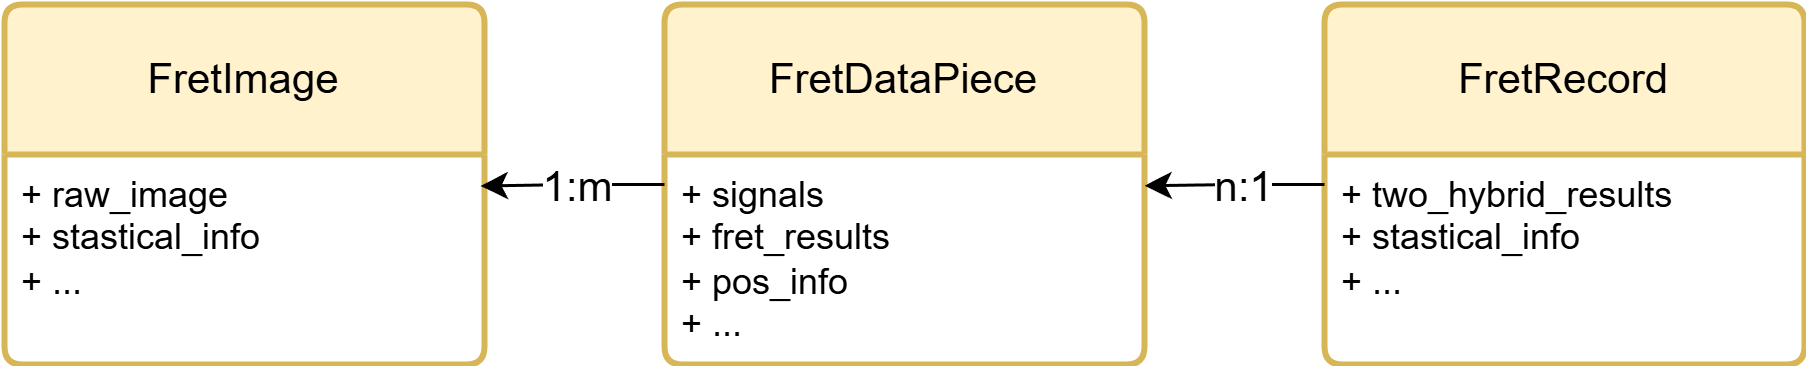
\includegraphics[width=1\linewidth]{../figures/2/2_Fretha数据层对应关系.png}
    \caption{Fretha数据层实体关联关系图}
    \label{fig:fretha_data_relations}
\end{figure}

\subsection{开发技术选型}
\ifshowtext
Qt 5.15.2是Qt官方发布的长期支持(LTS)版本,具有卓越的跨平台性能。该版本能够在Windows、Linux、macOS以及嵌入式系统等多种平台上稳定运行。
开发者只需对一套代码进行简单配置,即可实现不同平台的适配,这种特性大幅降低了软件开发与维护的成本。FRETscopeII的控制软件系统选择了Qt 5.15.2版本作为技术选型。
为了确保Fretha和FRETscopeII在开发过程中的一致性和可融合性,Fretha同样选用该版本作为软件开发的基础技术。
这一选择不仅有利于代码的共享、复用和维护,还能显著降低二次开发以及未来合并开发过程中的成本和风险。

在计算机视觉处理方面,Fretha选用了OpenCV(Open Source Computer Vision Library)。
OpenCV是一个开源的计算机视觉与机器学习软件库,具备强大的跨平台能力,可在Windows、Linux、macOS、Android、iOS等多种操作系统上运行。
其功能丰富多样,广泛涵盖了图像和视频处理的各个方面,例如图像的读取、滤波、边缘检测等。
在性能上,OpenCV经过SIMD指令集优化以及多线程并行计算等技术的优化,处理效率得到了显著提升,能够充分满足实时性的需求。
此外,OpenCV拥有一个活跃的社区,汇聚了大量的开发者。
社区中提供了丰富的算法、示例代码和实际案例,为开发者提供了有力的技术支持和学习借鉴的资源。
基于以上诸多优势,OpenCV完全契合本项目中计算机视觉任务的需求,因此被选定为本项目的重要技术工具。

在最优化计算方面,Fretha选择了C++库Dlib。
Dlib库集成了基于梯度的优化算法,并采用了自适应学习率机制,能够实现快速且稳定的收敛,有效降低了陷入局部最优解的概率。
该库还采用了牛顿法与拟牛顿法,在保证计算精度的同时兼顾了计算效率。
此外,Dlib在处理约束优化问题方面表现出色,例如可以运用内点法来解决资源分配中的约束难题,为研究工作提供了可靠的支持。  
\fi

\section{FRET算法和后台接口}

\subsection{FRET定量计算器}
FRET定量计算器(FretCalculator)用于处理E-FRET和$3^3$-FRET定量计算。FRET定量计算器定义了参数设置、数据加载、数据校正、数据计算和结果获取等计算步骤,每个步骤需要按照顺序执行,并且在执行时记录运行状态,在获取结果数据之前进行检查来保证数据安全。

\begin{figure}[hbtp]
  \centering
  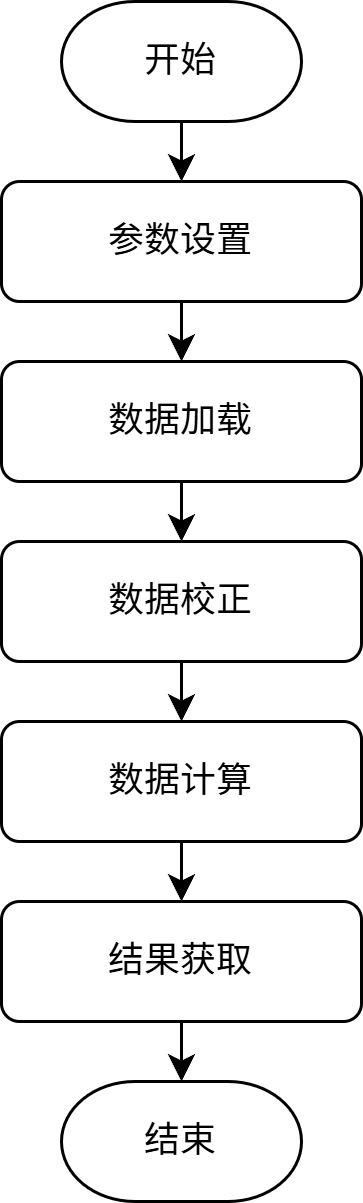
\includegraphics[width=0.25\linewidth]{../figures/2/2_FRET定量计算器流程.png}
  \caption{FretCalculator计算步骤}
  \label{fig:fretha_calculator}
\end{figure}

\subsection{FRET图像处理器}
FRET图像处理器(FretImageProcesser)封装了对FRET图像进行计算分析的计算器类,还静态方法的形式提供了图像处理算法的一系列接口。
首先按照FRET计算器的计算步骤对FRET图像数据进行处理,然后根据FRET图像数据的特点进行分析,完成逐像素的FRET计算,最后将计算结果保存到数据层中。
与FRET定量计算器不同,FRET图像分析时需要对每个像素点的荧光强度进行计算,因此需要对图像数据进行遍历处理。
FRET图像处理器采用OpenCV的Mat数据结构来存储图像数据。OpenCV提供的数据结构Mat是一个多维数组,可以方便地存储和处理图像数据,很适合存储逐像素的FRET图像数据。
FRET图像处理器的计算类FretImageProcesser的计算步骤和FRET定量计算器类似,如图 \ref{fig:fretha_calculator} 所示。

FRET图像处理器以静态方法的形式提供了FRET图像处理时涉及的一系列算法接口,包括图像预处理、图像分割、特征提取、图像增强等。所有的算法接口如表 \ref{tab:算法接口} 所示。
运用这些算法,FRET图像处理器支持了对16位原始数据的计算处理能力,以及可视化输出为伪彩图等功能。

\begin{table}[hbtp]
  \centering
  \caption{FRET图像处理库算法接口}
  \label{tab:算法接口}
    \begin{tabular*}{\textwidth}{p{0.3\textwidth}p{0.3\textwidth}p{0.4\textwidth}}
      \toprule[1.5pt]
      {\hei 接口} & {\hei 参数} & {\hei 说明} \\
      \hline

      morphologyClose & 
      \begin{tabular}[t]{@{}l@{}}
        Mat: 二值化图像 \\ 
        int: 迭代次数
      \end{tabular} & 
      形态学闭运算 \\

      morphologyOpen & 
      \begin{tabular}[t]{@{}l@{}}
        Mat: 二值化图像 \\ 
        int: 迭代次数
      \end{tabular} & 
      形态学开运算 \\
      
      medianFilter & 
      \begin{tabular}[t]{@{}l@{}}
        Mat: 单通道图像 \\ 
        int: 核大小
      \end{tabular} & 
      图像中值滤波 \\

      meanFilter & 
      \begin{tabular}[t]{@{}l@{}}
        Mat: 单通道图像 \\ 
        int: 核大小
      \end{tabular} & 
      图像均值滤波 \\
      
      gaussianFilter & 
      \begin{tabular}[t]{@{}l@{}}
        Mat: 单通道图像 \\ 
        int: 核大小 \\
        double: 高斯标准差
      \end{tabular} & 
      图像高斯平滑 \\
      
      getBackgroundValue & 
      Mat: 单通道图像 & 
      基于直方图的背景值估计 \\
      
      otsuThreshold & 
      \begin{tabular}[t]{@{}l@{}}
        Mat: 输入图像 \\ 
      \end{tabular} & 
      Otsu自动阈值分割 \\
      
      adaptiveThreshold & 
      \begin{tabular}[t]{@{}l@{}}
        Mat: 输入图像 \\ 
        int: 邻域大小(奇数) \\ 
        double: 阈值偏移量
      \end{tabular} & 
      自适应局部阈值分割 \\
      
      applyPseduoColor & 
      Mat: 单通道图像(8位) & 
      伪彩色映射(Jet颜色表) \\
      
      applyMask & 
      \begin{tabular}[t]{@{}l@{}}
        Mat: 输入图像 \\ 
        Mat: 掩膜(二值/同尺寸)
      \end{tabular} & 
      图像掩膜操作 \\
      
      minMaxNormalization & 
      Mat: 输入图像 & 
      全局线性归一化 \\
      
      mergeChannels & 
      \begin{tabular}[t]{@{}l@{}}
        Mat: R通道(8位) \\ 
        Mat: G通道(8位) \\ 
        Mat: B通道(8位)
      \end{tabular} & 
      多通道图像合并 \\
      \bottomrule[1.5pt]
    \end{tabular*}
\end{table}

\subsection{FRET双杂交求解器}
FRET 双杂交求解器对采集到的 FRET 批数据 $E_D$、$E_A$、$R_C$、$A_{est}$ 和 $D_{est}$ 进行最优化计算,以获取使预测结果与测量结果之间误差最小的$E_{A,max}$、$E_{D,max}$、$N_D / N_A$、$K_{d,EFF}$等参数。求解器从数据模型 FretRecord 中获取批量数据作为数据集,然后分别按照 DC-FRET 方法或 L-FRET 方法进行 FRET 双杂交分析求解。
具体算法如下:
\begin{enumerate}
  \item \textbf{DC-FRET线性拟合算法的封装}。根据公式\ref{eq:ea_appro}和\ref{eq:ed_appro},DC-FRET拟合斜率时截距项为0。以参数$E_{A,max}$的拟合过程为例,其线性方程形式为
  \begin{equation}
      E_D = E_{A,max}\cdot R_C,
  \end{equation}
  其中,$E_D$是自变量,$R_C$是自变量,$E_{A,max}$是斜率。线性拟合的目标是找到合适的参数$E_{A,max}$,使得方程预测的$E_D$值与实际观测到的$E_D$值之间的误差尽可能小。
  通常使用最小二乘法,其原理是最小化观测值与预测值之间的误差平方和,即
  \begin{equation}
      S=\sum^{n}_{i=1}(E_{D_i}-(E_{A,max}R_{C_i}))^2
  \end{equation}
  其中,$n$是数据点的数量,$R_{C_i}$和$E_{D_i}$分别是第i个数据点的自变量和因变量的值。
  为了找到$S$最小的$E_{A,max}$值,对$S$关于$E_{A,max}$求偏导,并令其等于0。
  首先,展开误差$S$:
  \begin{align}
       S=\sum_{i = 1}^{n}(E_{D_i}^{2}-2E_{A,max}R_{C_i}E_{D_i} + E_{A,max}^{2}R_{C_i}^{2}), \\
       \frac{\partial S}{\partial E_{A,max}}=\sum_{i = 1}^{n}(-2R_{C_i}E_{D_i} + 2E_{A,max}R_{C_i}^{2}),
  \end{align}
  令 \(\frac{\partial S}{\partial E_{A,max}}=0\):
  \begin{align}
       \sum_{i = 1}^{n}(-2R_{C_i}E_{D_i} + 2E_{A,max}R_{C_i}^{2}) = 0, \\
      -2\sum_{i = 1}^{n}R_{C_i}E_{D_i}+2E_{A,max}\sum_{i = 1}^{n}R_{C_i}^{2}=0,
  \end{align}
  最后求解$E_{A,max}$:
  \begin{equation}
         E_{A,max}=\frac{\sum_{i = 1}^{n}R_{C_i}E_{D_i}}{\sum_{i = 1}^{n}R_{C_i}^{2}}. \label{eq:linear_fit_quick}
  \end{equation}
  公式 \ref{eq:linear_fit_quick} 给出了线性拟合求解$E_{A,max}$的解析公式,应用类似方法可直接计算斜率$E_{A,max}$和$E_{D,max}$,从而避免了基于迭代的线性拟合求解算法的消耗。

  \item \textbf{L-FRET Langmiur模型拟合算法的封装。}Langmiur模型具有模型的非线性和参数的复杂性,无法通过简单的解析式解析其求解公式。因此,我们引入dlib计算库进行复杂的参数拟合。

  为完成拟合计算,需要设计专门的数据类型ColumnVector和ExperimentalData,如代码 \ref{code:data_type}所示。
  ColumnVector类型用于存储双精度浮点数的列向量,在后续的计算和优化过程中承载参数向量和中间计算结果。
  ExperimentalData结构体用于存储来自实验采集到的数据集,该结构体包含四个std::vector<double>类型的成员变量:aest存储$A_{est}$相关的数据数组,dest存储$D_{est}$相关的数据数组,ea\_corr存储$E_A$预测值($E_{A,p}$)与测量值($E_{A,o}$)之间的误差,ed\_corr存储$E_D$预测值($E_{D,p}$)与测量值($E_{D,o}$)之间的误差。
  \begin{lstlisting}[language=C++, caption={数据类型}, label={code:data_type}]  
  // 定义列向量类型
  typedef dlib::matrix<double, 0, 1> ColumnVector;
  
  // 定义数据结构体,用于存储实验数据
  struct ExperimentalData {
      std::vector<double> aest;
      std::vector<double> dest;
      std::vector<double> ea_corr;
      std::vector<double> ed_corr;
  };
  \end{lstlisting}
  如代码 \ref{code:error_calculate} 所示,CalculateLoss函数负责计算模型在整个数据集上的整体损失。
  对于给定的ExperimentalData实例data和参数向量parameters,CalculateLoss函数首先遍历数据集中的每个数据点,计算出$E_A$或$E_D$预测值和与实际值之间的误差,最后将误差累加到total\_error中。
  \begin{lstlisting}[language=C++, caption={误差计算函数}, label={code:error_calculate}]
  // 计算整体损失
  double CalculateLoss(const ExperimentalData& data, const ColumnVector& parameters) {
      double total_error = 0.0;
      for (size_t i = 0; i < data.aest.size(); ++i) {
          double d_free = ((data.dest[i] - parameters(0) - data.aest[i] * parameters(1)) + std::sqrt(std::pow(data.dest[i] - parameters(0) - data.aest[i] * parameters(1), 2) + 4 * parameters(0) * data.dest[i])) / 2;
          double a_free = data.aest[i] - (data.dest[i] - d_free) / parameters(1);
          double ea_pred = parameters(2) * d_free / (d_free + parameters(0));
          double ed_pred = parameters(3) * a_free / (a_free + parameters(0) / parameters(1));
  
          total_error += CalculateError(data.ea_corr[i], ea_pred) + CalculateError(data.ed_corr[i], ed_pred);
      }
      return total_error;
  }
  \end{lstlisting}
  TwoHybridSolver是用来调用整个拟合过程的函数,并向外提供调用接口,如代码 \ref{code:two_hybrid_solver} 所示。
  {TwoHybridSolver} 函数接受四个 std::vector<double> 类型的参数,分别为 {aest\_data}、{dest\_data}、{ea\_corr\_data} 和 {ed\_corr\_data},返回一个 {ColumnVector} 类型的对象,其中存储了经过拟合的结果参数。整个拟合过程如下:
  首先设置$K_{d,EFF}$、$n_D/n_A$、$E_{A,max}$和$E_{D,max}$的拟合初值为 1、1、0.5 和 0.5, 存储到{ColumnVector} 对象 {starting\_point},作为参数拟合的起始点。
  创建一个 {ExperimentalData} 类型的对象 {data},将传入的四个实验数据向量存储在该结构体中,以便后续目标函数使用。
  使用 {dlib} 库中的 {find\_min\_using\_approximate\_derivatives} 函数进行优化。
  在搜索策略算法上,求解器采用一种拟牛顿法 {dlib::bfgs\_search\_strategy()} ,用于在参数空间中寻找目标函数的最小值,并使用 {dlib::objective\_delta\_stop\_strategy(1e - 7)} 作为停止策略,当两次拟合后参数的变化小于 $10^{-7}$ 时,认为此时的结果已收敛,停止优化过程。
  最后,函数返回 {starting\_point},此时 {starting\_point} 存储的是经过优化后得到的拟合参数。
  \begin{lstlisting}[language=C++, caption={双杂交求解器}, label={code:two_hybrid_solver}]
    
    // 双杂交求解器,进行参数拟合
    ColumnVector TwoHybridSolver(const std::vector<double>& aest_data, const std::vector<double>& dest_data, const std::vector<double>& ea_corr_data,const std::vector<double>& ed_corr_data) {
        // 初始化起始点
        ColumnVector starting_point(4);
        starting_point = 1, 1, 0.5, 0.5;
    
        // 创建数据结构体
        ExperimentalData data = {aest_data, dest_data, ea_corr_data, ed_corr_data};
    
        // 定义目标函数包装器
        auto objective_wrapper = [&data](const ColumnVector& parameters) {
            return ObjectiveFunction(parameters, &data);
        };
    
        // 使用 dlib 进行优化
        dlib::find_min_using_approximate_derivatives(dlib::bfgs_search_strategy(), dlib::objective_delta_stop_strategy(1e-7), objective_wrapper, starting_point, -1, 0.01);
  
        return starting_point;
    }
    \end{lstlisting}  
\end{enumerate}

\section{功能模块的实现}

\subsection{成像参数设置模块}
\ifshowtext
FRET定量分析中,在数据处理前需要设置好FRET定量计算过程中必须的参数,设置成像过程时的成像参数至关重要。
成像参数设置模块的界面如图 \ref{fig:参数设置页界面} 所示,包括了FRET成像参数的设置和保存功能。

FRET成像参数在Fretha中以静态参数保存在软件内存中,是数据处理时的环境参数。其中,a、b、c、d、G、k和Y是FRET成像系统的光学参数,在前文中已介绍;ExpTimeAA、ExpTimeDD和ExpTimeDA是成像时三个探测通道的曝光时间,在FRET定量计算时需要根据曝光时间参数在各个通道归一化,然后才能进行计算。
Fretha中包括的所有成像参数如表 \ref{tab:fretha_param_list} 所示。

\begin{table}[htb]
  \centering
  \caption[FRET成像参数]{FRET成像参数}
  \label{tab:fretha_param_list}
    \begin{tabular*}{\textwidth}{cp{8cm}lc}
      \toprule[1.5pt]
      {\hei 参数} & {\hei 说明} & {\hei 意义范围} & {\hei 单位} \\
      \hline
      \text{a} & 供体激发时在DA通道的串扰系数 & $(0,1)$ & 无\\
      \text{b} & 所有的一切都在这里面。 & $(0,1)$ & 无\\
      \text{c} & 模板类文件。 & $(0,1)$ & 无\\
      \text{d} & 受体激发时在DA通道的串扰系数 & $(0,1)$ & 无\\
      \text{G} & 供体猝灭和受体荧光增强的比值         & $(0,+\infty)$ & 无\\
      \text{k} & 受体浓度和供体浓度相同时的荧光比值 & $(0,+\infty)$ & 无\\
      \text{Y} & 供受体在激发光条件下的消光系数之比,也记作$\varepsilon_{YFP}(\lambda)/\varepsilon_{CFP}(\lambda)$   & $(0,+\infty)$ & 无\\
      \text{ExpTimeDD} & DD通道下的成像曝光时间 & $(0,+\infty)$ & 毫秒(ms)\\
      \text{ExpTimeDA} & DA通道下的成像曝光时间 & $(0,+\infty)$ & 毫秒(ms)\\
      \text{ExpTimeAA} & AA通道下的成像曝光时间 & $(0,+\infty)$ & 毫秒(ms)\\
      \bottomrule[1.5pt]
    \end{tabular*}
\end{table}

参数设置业务设计上遵循一定的原则。首先,设置时所有参数应一同更新,避免因参数不匹配导致的数据处理错误。其次,每个参数需要在其有意义的范围内,避免无意义的值。
因此,在点击“更新参数”按钮时,若无法从界面中的每个参数输入框都解析到合法的数字,那么本次更新参数就会失败。
FRET成像参数是一批参数,参数间存在依赖关系,如测量参数$G$、$k$、$Y$就依赖参数$a$、$b$、$c$、$d$,这是因为测定参数$G$、$k$、$Y$时需要计算敏化发射荧光$F_C$,根据公式 \ref{eq:fc} 所示,$F_C$的确定与$a$、$b$、$c$、$d$密切相关。
强制所有参数一同更新可以避免用户单独设置某一参数而导致参数之间不匹配等问题。

FRET成像参数一般比较稳定,一般2到3个月才需要重新测量,因此需要持久化到本地,以供多次处理数据时使用。
Fretha的本地参数文件保存为可执行程序同级目录下的“config.ini”中。在软件初始化阶段,会自动检测并应用本地配置文件中的参数。
用户可通过保存多套配置文件,在使用时替换目标配置文件,快速进行参数配置的切换。

参数设置的主要业务流程如图 \ref{fig:fretha_param_module_flow} 所示。

\begin{figure}[hbtp]
    \centering
    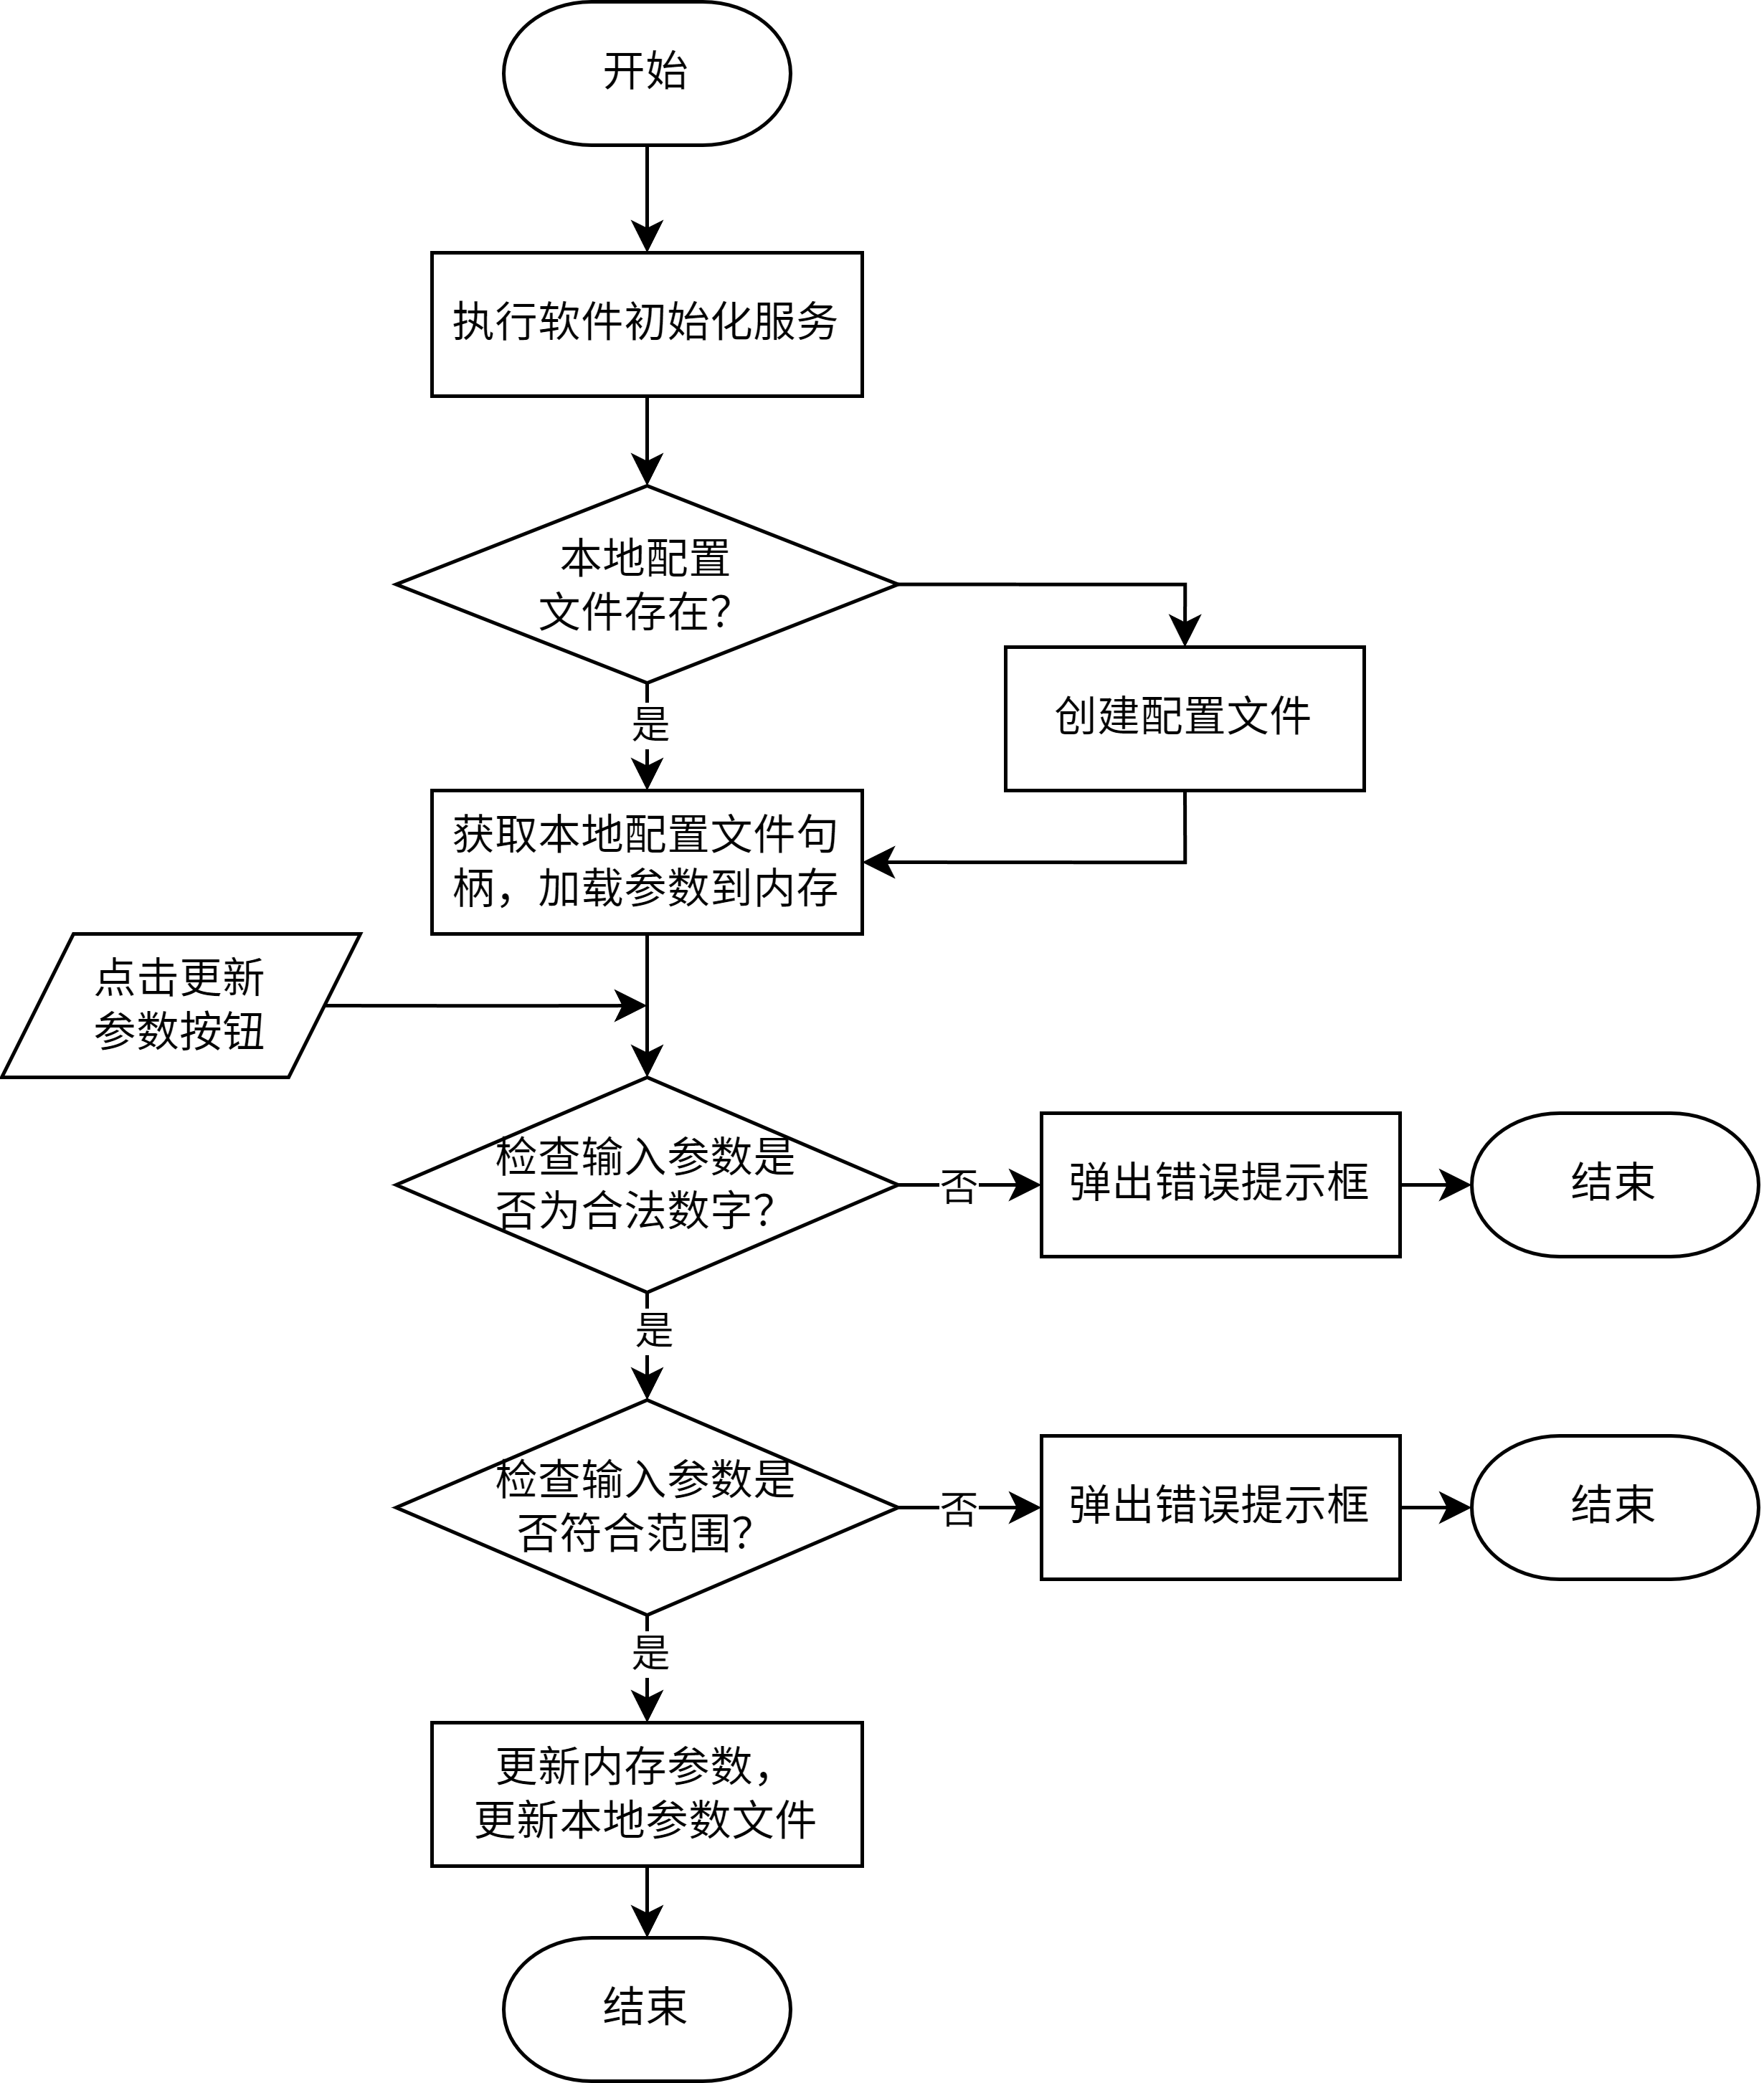
\includegraphics[height=1\linewidth]{../figures/2/2_成像参数设置模块业务流程.png}
    \caption{参数设置模块业务流程}
    \label{fig:fretha_param_module_flow}
\end{figure}
\fi

\subsection{数据检验模块}
\label{sec:数据检验模块}

FRET双杂交分析需要处理一批FRET图像文件,因此需要对输入数据的完备性进行检验识别。
该模块的作用有以下两个方面:一方面通过模式识别FRET合法数据,避免了异常输入导致的运行错误;
另一方面,在这一模块会将FRET批数据的视野子文件夹进行解析和类型识别,为后续数据处理提供对子文件夹的不同操作。

Fretha的数据识别检验模块匹配识别FRETscopeII的数据格式,从而保证数据处理能够正常开始。
如图 \ref{fig:fretscope_data_struct} 所示,FRETscopeII的数据结构由上层到下层依次为:
\begin{enumerate}
  \item 批数据根目录:存放所有视野子目录和数据文件;
  \item 视野子目录:存放一个视野的三通道图片和参数文件;
  \item 图片数据和参数文件。
\end{enumerate}

\begin{figure}[htbp]
    \centering
    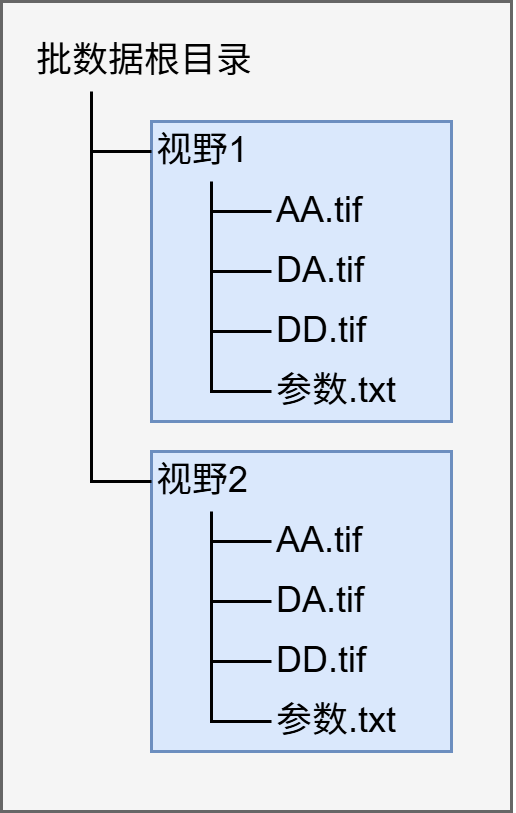
\includegraphics[height=0.5\linewidth]{../figures/2/2_FRETscopeII数据格式.drawio.png}
    \caption{FRETscopeII数据文件结构}
    \label{fig:fretscope_data_struct}
\end{figure}

数据检验业务的流程如图 \ref{fig:fretha_data_check_flow} 所示。
其中,检查子文件夹类型是通过图 \ref{fig:fretscope_data_struct} 进行匹配的,当且仅当子文件夹中同时存在“DA.tif”、“DD.tif”和“AA.tif”图片文件时,当前子文件夹会被识别为FRET视野,并在视野表格模型中记录。
其他情况的子文件夹会被记作“Unknown”文件夹,在后续FRET图像处理或者自动处理中被跳过。
这种检查还会对图像数据是否可读进行检查。
\begin{figure}[htbp]
    \centering
    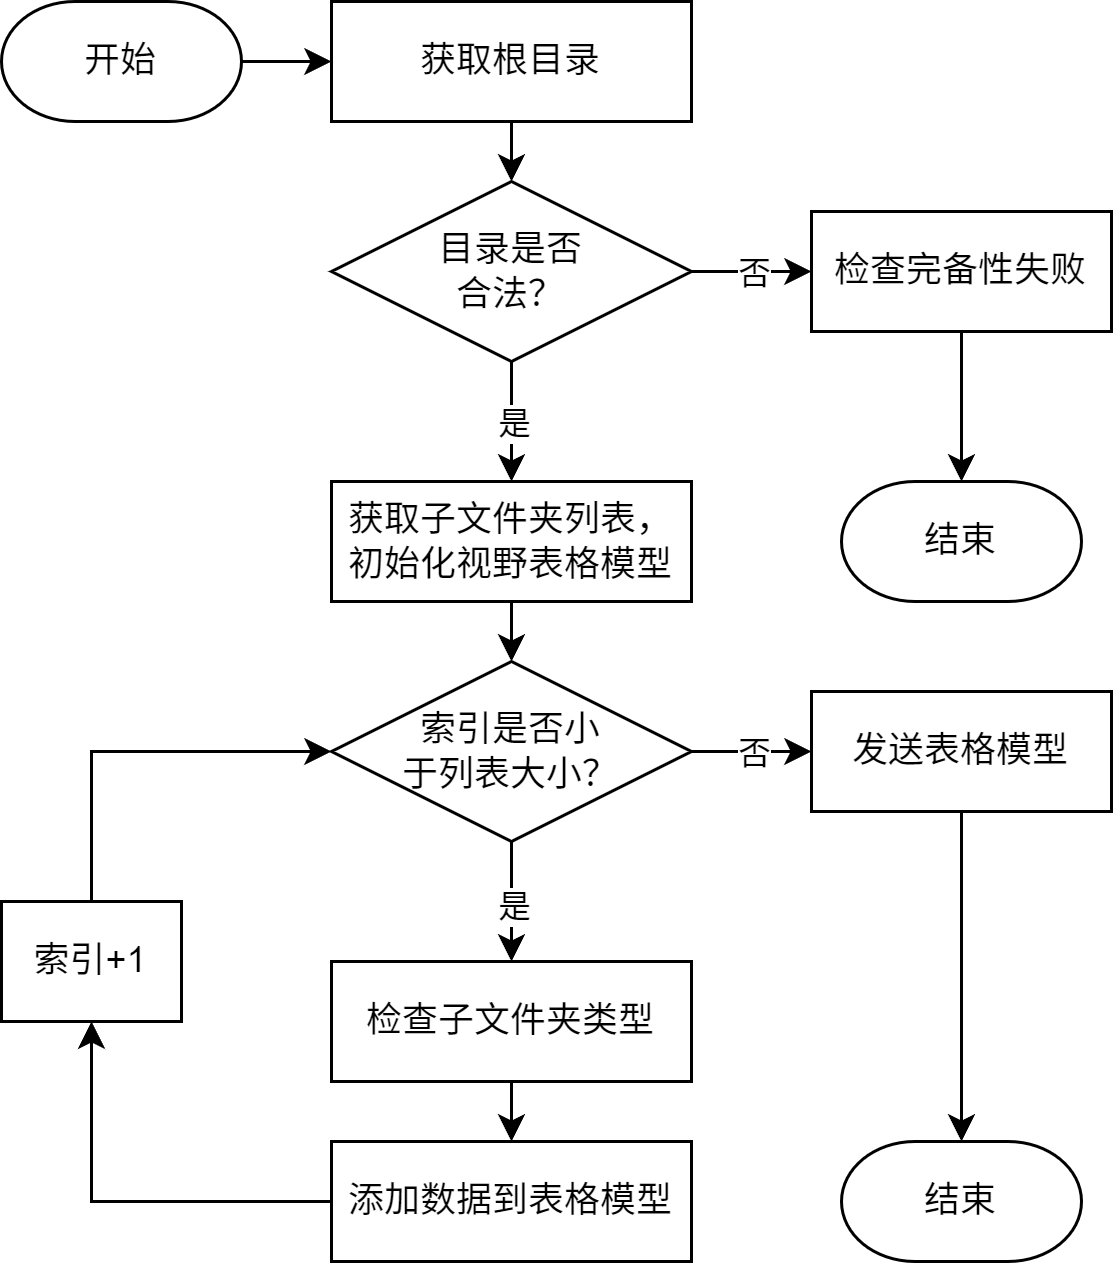
\includegraphics[width=0.6\linewidth]{../figures/2/2_数据完备性检验业务.drawio.png}
    \caption{Fretha数据检验业务主流程图}
    \label{fig:fretha_data_check_flow}
\end{figure}
\subsection{FRET图像处理模块}
\label{sec:FRET图像处理模块}
FRET图像处理模块是对FRET三通道图像进行ROI提取等图像处理分析的模块,包括手动ROI圈点和自动ROI圈点等。其界面如图 \ref{fig:fretha_imageprocess_ui} 所示:
\begin{figure}[htbp]
    \centering
    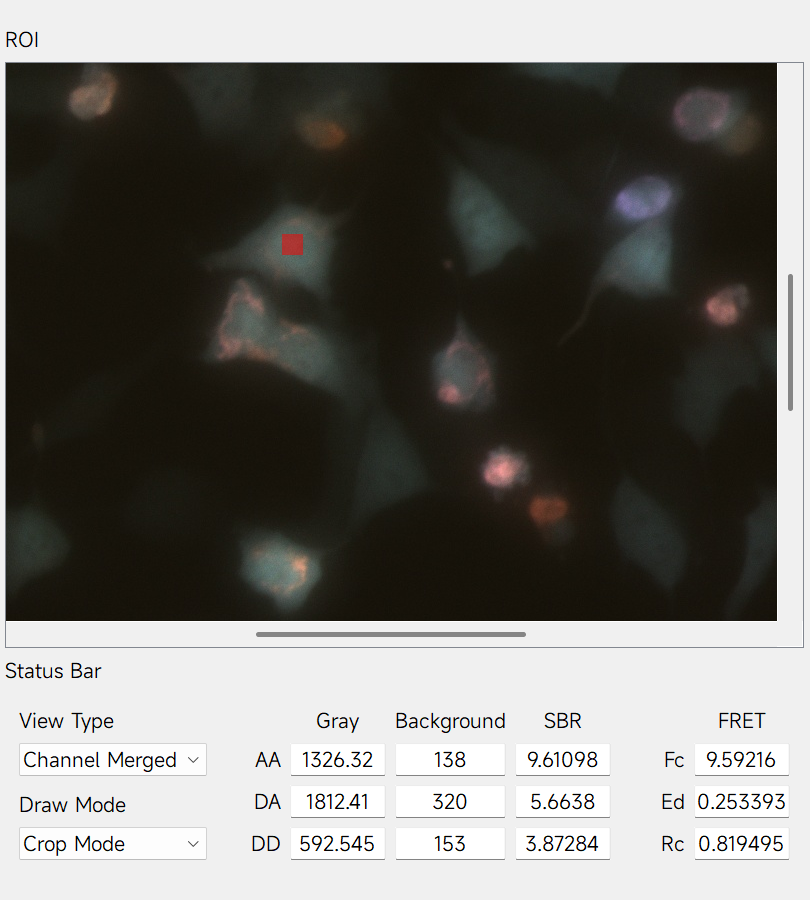
\includegraphics[width=0.75\linewidth]{../figures/2/2_图像处理模块界面.png}
    \caption{Fretha图像处理模块界面}
    \label{fig:fretha_imageprocess_ui}
\end{figure}
在FRET图像处理工作里,手动选取感兴趣区域ROI是一个基础且关键的操作,它能帮助分析人员聚焦于特定区域,进行更精确的数据处理与分析。
为实现图像处理过程中 ROI 的手动选取功能,Fretha 借助 Qt 框架提供的 QGraphicsView 类,开发了自定义的 FretGraphicsView 类。
QGraphicsView 是 Qt 用于可视化和交互处理二维图形场景的重要类,具备丰富的功能和良好的可扩展性,为 FretGraphicsView 的实现提供了有力支撑。

FretGraphicsView 类中设计了一个基于QRectItem的ROI 成员,它能够在视图中直观呈现 ROI 的大小和位置,方便用户确认所选区域。
设定ROI的绘制模式为“Crop Mode”截取模式时,此时会根据鼠标和ROI边框的位置,变换ROI交互的功能,包括ROI的创建、移动、缩放等操作。
切换绘制模式为“Stamp”邮戳模式,此时可以固定ROI的大小,从而快速圈选多个大小一致的ROI。

Fretha的状态栏中提供了视图类型切换选项,在数据处理中可以辅助圈点,支持的视图类型如表\ref{tab:fretha_viewtype_list}所示。
\begin{table}[htbp]
  \centering
  \caption[FRET图像视图类型]{FRET图像视图类型表}
  \label{tab:fretha_viewtype_list}
    \begin{tabularx}{\linewidth}{
    >{\centering\arraybackslash}X
    >{\centering\arraybackslash}X
    >{\centering\arraybackslash}X
    >{\centering\arraybackslash}X
    >{\centering\arraybackslash}X
    >{\centering\arraybackslash}X} % 修改第二列格式为p{6cm},可根据实际情况调整宽度
      \toprule[1.5pt]
      {\hei 信息} & {\hei 说明} \\
      \hline
      Channel Merged & 三通道归一合成图 \\
      DD Normalized & DD通道的归一化增强图 \\
      DA Normalized & DA通道的归一化增强图 \\
      AA Normalized & AA通道的归一化增强图 \\
      $R_C$ Pseudo & $R_C$逐像素数值伪彩图 \\
      $E_D$ Pseudo & $E_D$逐像素数值伪彩图 \\
      \bottomrule[1.5pt]
    \end{tabularx}
\end{table}
归一化增强图包括DD、DA、AA通道分别归一化的增强视图以及三通道归一化合成图。
由于FRET成像系统的相机的量程为$[0,65535]$,计算机显示渲染机制里显示会将65535的灰度值设为白色,而0的灰度值设为黑色,这样会导致图像的对比度不高,不利于观察。
通过表 \ref{tab:算法接口} 中的 minMaxNormalization 算法,可以对图像进行全局线性归一化,从而增强图像的对比度。
三通道归一化合并图则是将三个通道的归一化增强图分别作为RGB色彩通道,合并成一幅彩色图像,以便于用户直观地观察三通道的信号分布情况。
增强视图的算法首先通过FretImageProcessor进行逐像素FRET计算得到$E_D$和$R_C$的逐像素矩阵,然后归一化后赋予伪彩图。

Fretha状态栏能够清晰展示当前视野及ROI的状态信息,如当前视野的三通道背景灰度值、ROI信号的三通道信号背景比等,还可以显示使用当前ROI提供的扣除背景灰度值后的$I_{DD}$、$I_{DA}$和$I_{DD}$,其中所有显示内容如表\ref{tab:fret_statusbar_list}所示。
FretGraphicsView 通过自定义鼠标释放事件的信号,实现了与数据访问层的数据交互。
当用户完成 ROI 选取并释放鼠标时,FretGraphicsView 会将 ROI 的坐标和大小信息传递给数据访问层。
数据访问层依据当前视野索引,从数据模型中读取相应的三通道图像文件,并且从ROI信息提取FRET信号。
在获得了$I_{DD}$、$I_{DA}$和$I_{DD}$后,Fretha后台会自动扣除每个通道的背景灰度,然后根据公式\ref{eq:fc},调用后台的FretCalculator计算出敏化发射的荧光强度$F_C$、$E_D$,$R_C$,并显示在状态栏中,方便用户获取处理结果,为ROI的保留和移除提供判断依据。
这种基于 QGraphicsView 扩展的设计,有效提升了 ROI 选取的灵活性和准确性。 

\begin{table}[htbp]
  \centering
  \caption[FRET圈点状态栏显示内容]{FRET圈点状态栏显示内容}
  \label{tab:fret_statusbar_list}
      \begin{tabular}{cc}
      \toprule
      {信息} & {说明} \\
      \hline
      DD通道信号 & DD通道的ROI内灰度均值 \\
      DA通道信号 & DA通道的ROI内灰度均值 \\
      AA通道信号 & AA通道的ROI内灰度均值 \\
      DD通道背景 & DD通道的视野背景灰度值 \\
      DA通道背景 & DA通道的视野背景灰度值 \\
      AA通道背景 & AA通道的视野背景灰度值 \\
      DD通道SBR & DD通道的信号背景比 \\
      DA通道SBR & DA通道的信号背景比 \\
      AA通道SBR & AA通道的信号背景比 \\
      $F_C$ & 敏化发射的荧光强度 \\
      $E_D$ & 供体视角的表观FRET效率 \\
      $R_C$ & 受体与供体的浓度比 \\
      \bottomrule
    \end{tabular}
\end{table}
点击左侧“自动圈点”按钮,可以使用LURS算法进行自动ROI圈点生成,并记录到右侧的数据区中。
计算过程中,Fretha界面通过进度条显示计算进度,方便用户查看。
自动圈点功能通过FRET双杂交求解器中封装的多线程服务,在不影响Fretha前台界面显示和操作的前提下,实现了一键式线程分离的自动数据处理。
自动ROI圈点模块的业务流程及架构如图\ref{fig:fret_auto_roi_flow}所示。
架构层内的流程流转以实线表示,不同架构层之间的流程流转以虚线表示。
在实现自动圈点功能的流程转移中,发生在架构不同层之间的转移占更多数,而层内的流程转移相对较少,分层架构设计使得每个层内实现较好的封装,因此能够在实现复杂业务功能时,只需要专注于层和层之间的数据和流程切换即可。
LURS算法将会在第三章具体说明。
\begin{figure}[htbp]
    \centering
    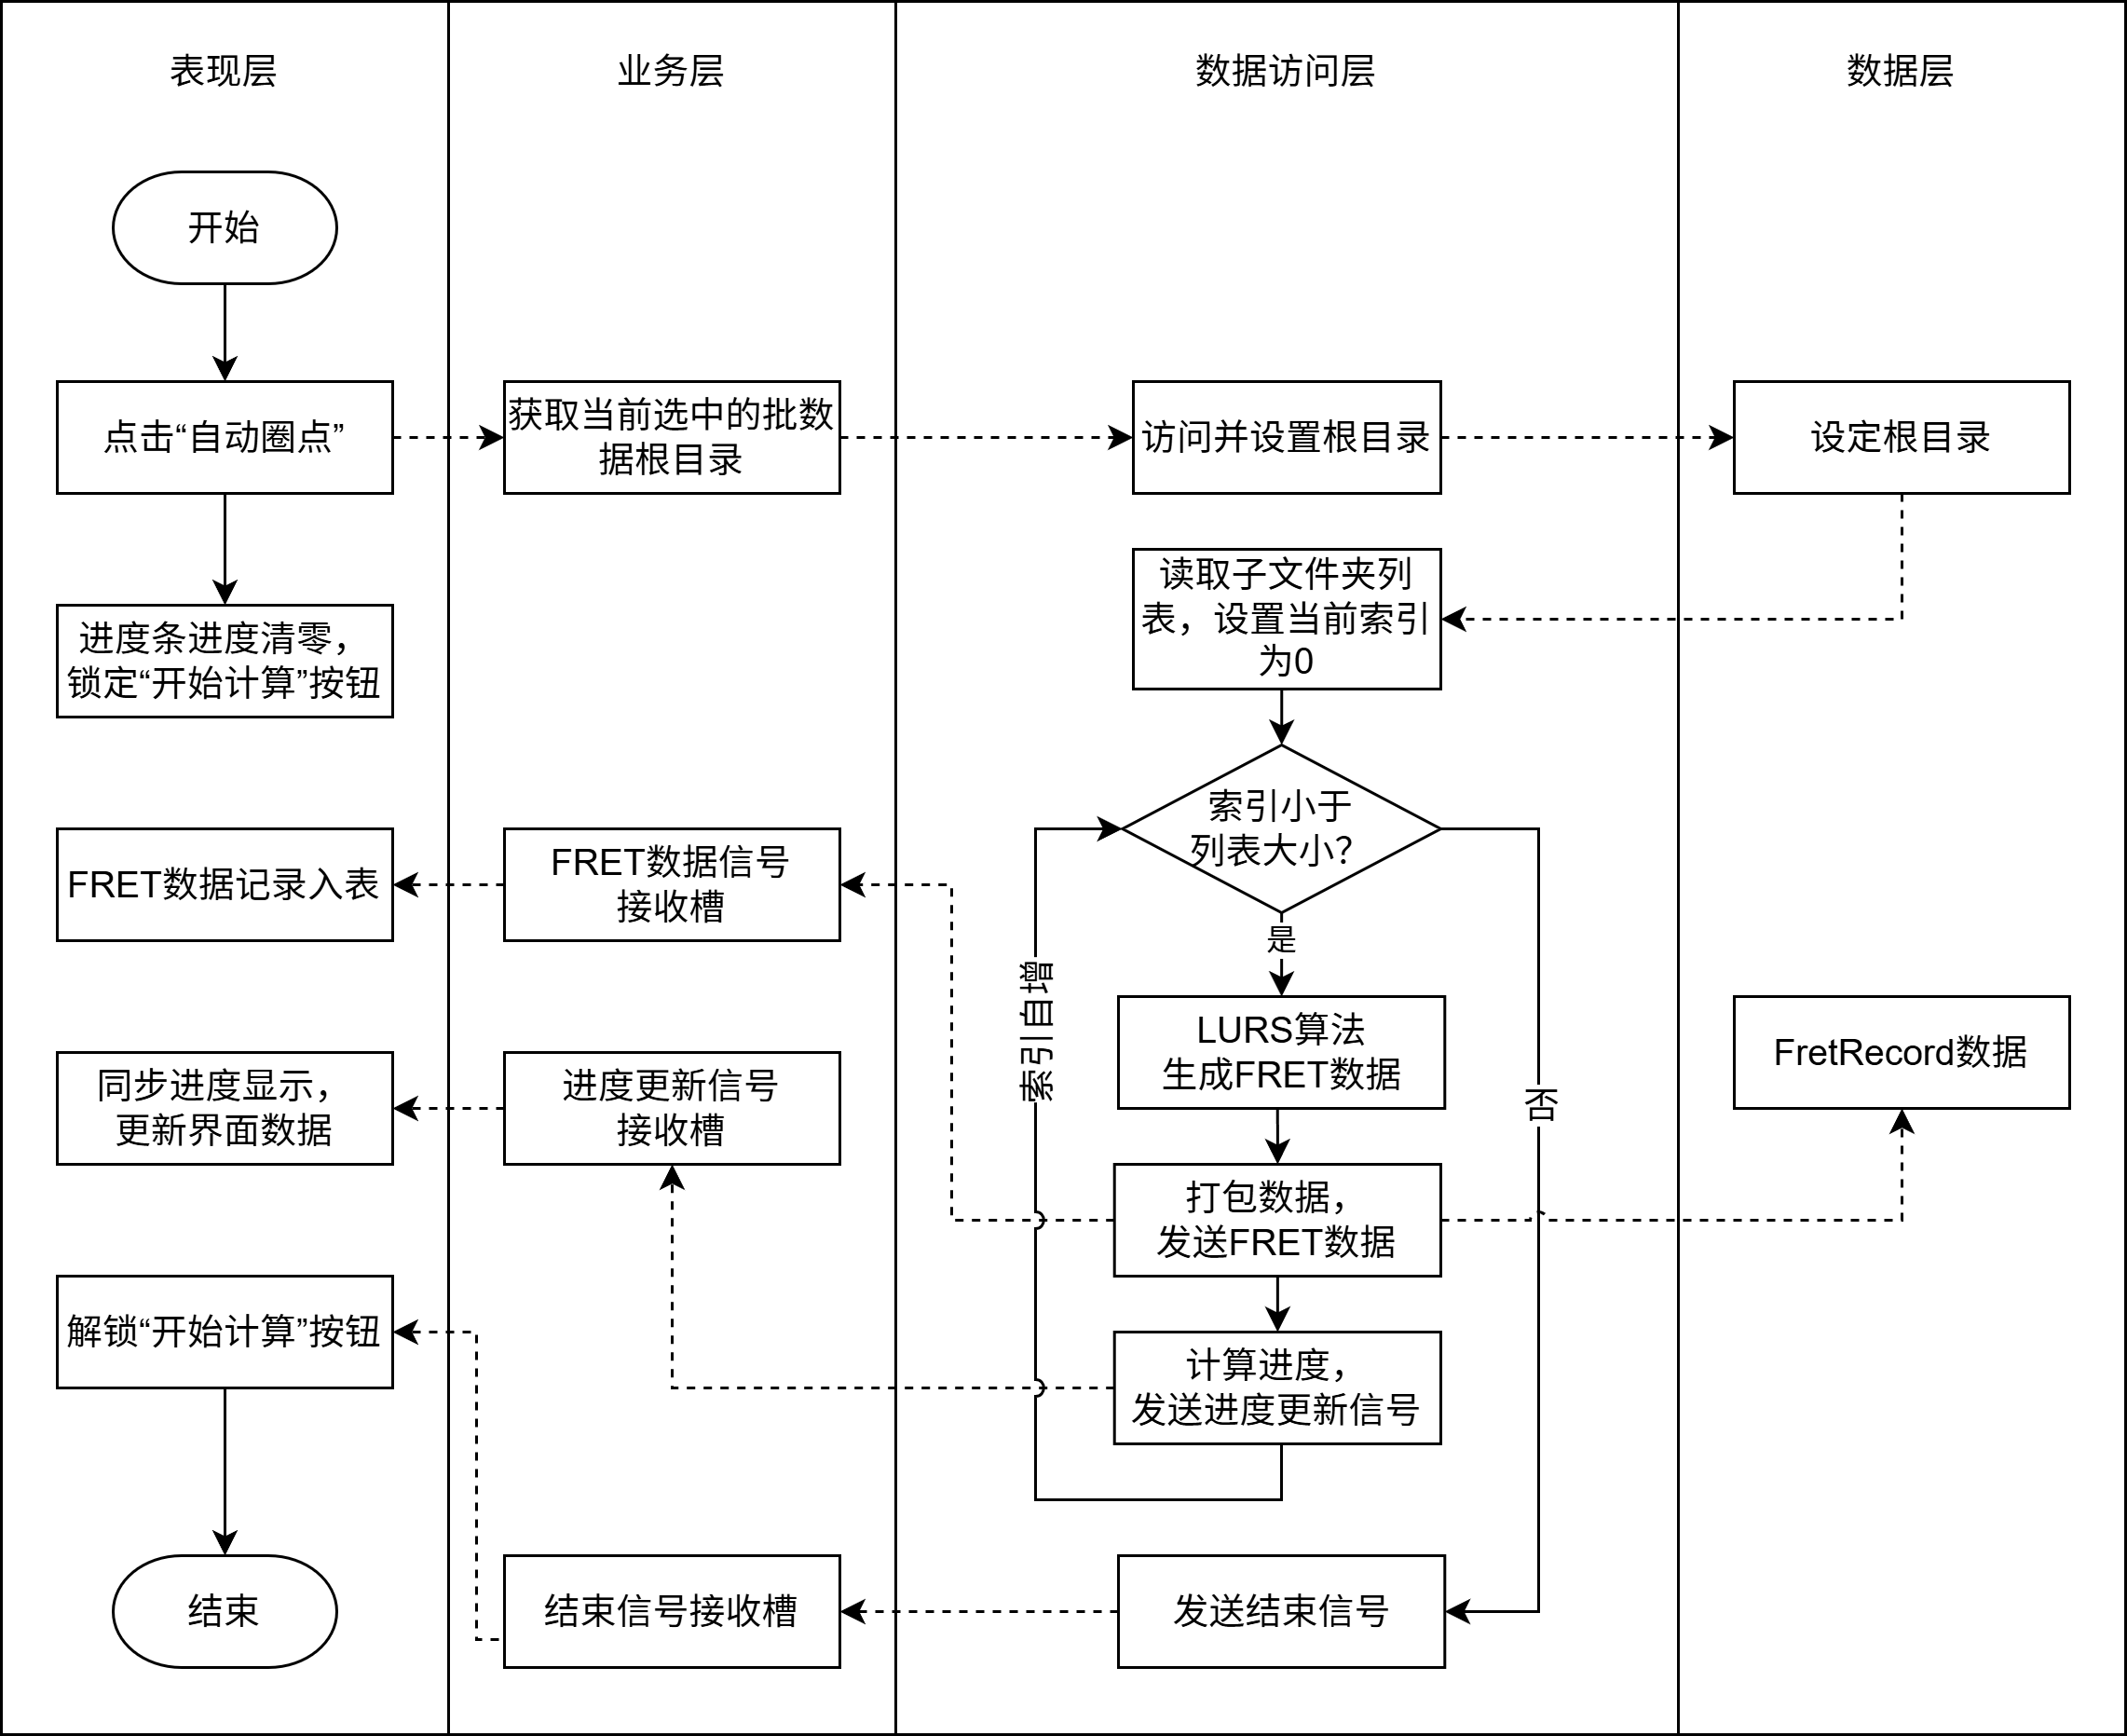
\includegraphics[width=1\linewidth]{../figures/2/2_自动ROI圈点模块业务流程.png}
    \caption{Fretha自动圈点模块流程}
    \label{fig:fret_auto_roi_flow}
\end{figure}

\subsection{数据管理模块}
\label{sec:数据管理模块}

数据管理模块支持对数据的实时操作,可以对于图像处理模块获得的数据,进行异常数据筛选、数据追踪、数据导入、数据导出、计算入口等数据管理控制功能。

一条数据类型FretDataPiece中包含数据如表 \ref{tab:数据项内容定义} 所示。
可以看出,FretDataPiece包含了一个ROI对应的所有原始信息,如ROI的位置、大小、信号强度、视野等;
同时,还包含了计算后的$E_D$、$E_A$、$R_C$、$1/R_C$等中间参数,可以直接被用于后续的数据处理。

\begin{table}[htbp]
  \centering
  \caption{FretDataPiece数据类型}
  \label{tab:数据项内容定义}
    \begin{tabular}{cc}
      \toprule
      {\hei 信息} & {\hei 说明} \\
      \hline
      $I_{DD}$ & ROI在DD通道扣除背景后的信号强度 \\
      $I_{DA}$ & ROI在DA通道扣除背景后的信号强度 \\
      $I_{AA}$ & ROI在DD通道扣除背景后的信号强度 \\
      $E_D$ & 根据$I_{DD}$、$I_{DA}$、$I_{AA}$计算的$E_D$ \\
      $R_C$ & 根据$I_{DD}$、$I_{DA}$、$I_{AA}$计算的$R_C$ \\
      $E_A$ & 根据$I_{DD}$、$I_{DA}$、$I_{AA}$计算的$E_A$ \\
      $1/R_C$ & $R_C$的倒数 \\
      $A_{est}$ & 供体相对分子数的估计值 \\
      $D_{est}$ & 受体相对分子数的估计值 \\
      $x$ & ROI的横坐标 \\
      $y$ & ROI的纵坐标 \\
      $w$ & ROI的宽度 \\
      $h$ & ROI的高度 \\
      $view$ & ROI隶属的视野\\
      \bottomrule
    \end{tabular}
\end{table}

为保证数据符合实际物理意义,避免中间变量的异常值对后续计算产生影响,数据管理模块提供了数据筛选功能。
点击“筛选数据”,数据管理模块会对数据根据物理定义和统计学准则进行筛选,剔除异常数据。
具体数据筛选流程实施如下:
\begin{enumerate}
  \item 对$I_DD$、$I_DA$、$I_AA$基于物理约束的初步数据清洗:
    针对各数值型变量 \( X_i \),依据其预设的物理合理区间 \( [L_i, U_i] \) 执行有效性校验。构建如下二元判别函数:
    \begin{equation}
      \delta(x_i) = 
      \begin{cases} 
        1, & x_i \notin [L_i, U_i] \\
        0, & x_i \in [L_i, U_i]
      \end{cases}
    \end{equation}
    当 \( \delta(x_i) = 1 \) 时,判定该数据点为物理意义上的异常值并予以剔除。
  \item 对中间变量$E_D$、$E_A$、$R_C$统计离群点检测:
    对经初步清洗后的数据子集 \( E_D \)、\( E_A \)和$R_C$,分别计算变量的样本均值 \( \mu \) 和样本标准差 \( \sigma \),计算公式如下:
    \begin{equation}
      \mu = \frac{1}{n}\sum_{i=1}^n x_i, \quad \sigma = \sqrt{\frac{1}{n - 1}\sum_{i=1}^n (x_i - \mu)^2}
    \end{equation}
    采用3σ准则设定离群阈值,即构建判别区间 \( [\mu - 3\sigma, \mu + 3\sigma] \)。超出该区间的观测值均判定为统计离群点并剔除。
\end{enumerate}

数据导出用于保存数据处理时的ROI信息。
在完成FRET图像处理和ROI绘制选取后,需要保存ROI的结果,以便后续分析或者修改编辑。
在数据管理模块点击“导出数据”按钮,Fretha将会导出数据区记录的所有数据,每一条数据都会按照FretDataPiece定义进行逐列导出,如表 \ref{tab:数据项内容定义} 所示,文件格式为CSV文件。
数据导入功能可以选择CSV文件,然后解析其中的数据按照FretDataPiece的格式。

点击“添加数据”按钮或者使用快捷键“A”,可以添加当前状态栏中的数据到数据表格中;
点击“删除数据”按钮或者使用快捷键“D”,可以删除数据表格中选中的数据;
点击“清空数据”按钮或者使用快捷键“C”,可以清空数据表格中的所有数据;
点击“开始计算”按钮,软件将调用FretTwoHybridSolver等算法对数据表格中的数据进行FRET双杂交分析求解计算,并将结果显示在结果可视化模块中,然后切换软件界面到结果可视化模块。

在数据表格中点击某一条数据,软件会根据这条数据的位置和形状信息,在图像显示上显示该条数据对应的ROI位置,以方便识别数据中潜在的错误。
实现这一功能,主要基于Qt提供的信号与槽机制。
将数据中的数据模型被点击的事件信号与FretGraphicsView控件中的回调槽函数绑定后,FretGraphicView模型可以接收到来自所选数据的信息,并将当前活动的ROI按照所选数据项中的信息$x$、$y$、$w$和$h$绘制到FretGraphicsView控件上。
接下来,FretGraphicsView会将窗口的视角移动到所选数据的ROI位置,以便用户更加直观地查看数据的位置和形状。

\subsection{结果可视化模块}
\label{sec:结果可视化模块}
\ifshowtext
FRET双杂交分析的输出结果包含双杂交计算的参数结果与拟合曲线图。
其中,$n_D/n_A$、$K_{d,EFF}$等参数作为表征生物大分子相互作用的核心量化指标,为生物学研究提供关键数据支撑。
拟合曲线图通过将双杂交理论拟合曲线与实验散点数据同图可视化,实现对拟合效果的直观评估,进而验证FRET双杂交分析结果的可靠性。

结果可视化模块的界面组成如图 \ref{fig:fretha_result_ui} 所示,主要包含以下三个功能区域:
\begin{enumerate}
  \item 视图选择:切换FRET双杂交分析算法,更新对应的结果视图;
  \item 图表分析:显示FRET双杂交分析的拟合趋势线和散点图;
  \item 操作按钮:结果保存按钮和返回圈点界面按钮。
\end{enumerate}

点击视图按钮可以切换不同FRET双杂交分析的算法方法的计算结果,更新图表分析区域显示的方法。
在可视化结果展示区域,软件将拟合结果与实验数据同步呈现在同一坐标系中,便于用户进行直接比对。
拟合曲线是基于拟合参数计算得到的理论数据点连接而成的平滑曲线,实验数据则以离散点形式展示,用户可以直观检查拟合计算的效果和误差大小。
可视化界面基于QChart组件作图绘制,根据一批数据(FretDataRecord)的数据范围分布,自动优化坐标轴刻度范围,以提升数据可视化的清晰度。

在 L-FRET 视图模式下,软件集成了数据预处理 BIN 功能,允许用户通过设定 BIN 的上下限及间隔参数,对数据合并预处理的参数进行灵活调节,然后点击“更新”按钮即可更新结果,在L-FRET计算效果不理想时可以用来优化数据处理结果。

\begin{figure}[htbp]
  \centering
  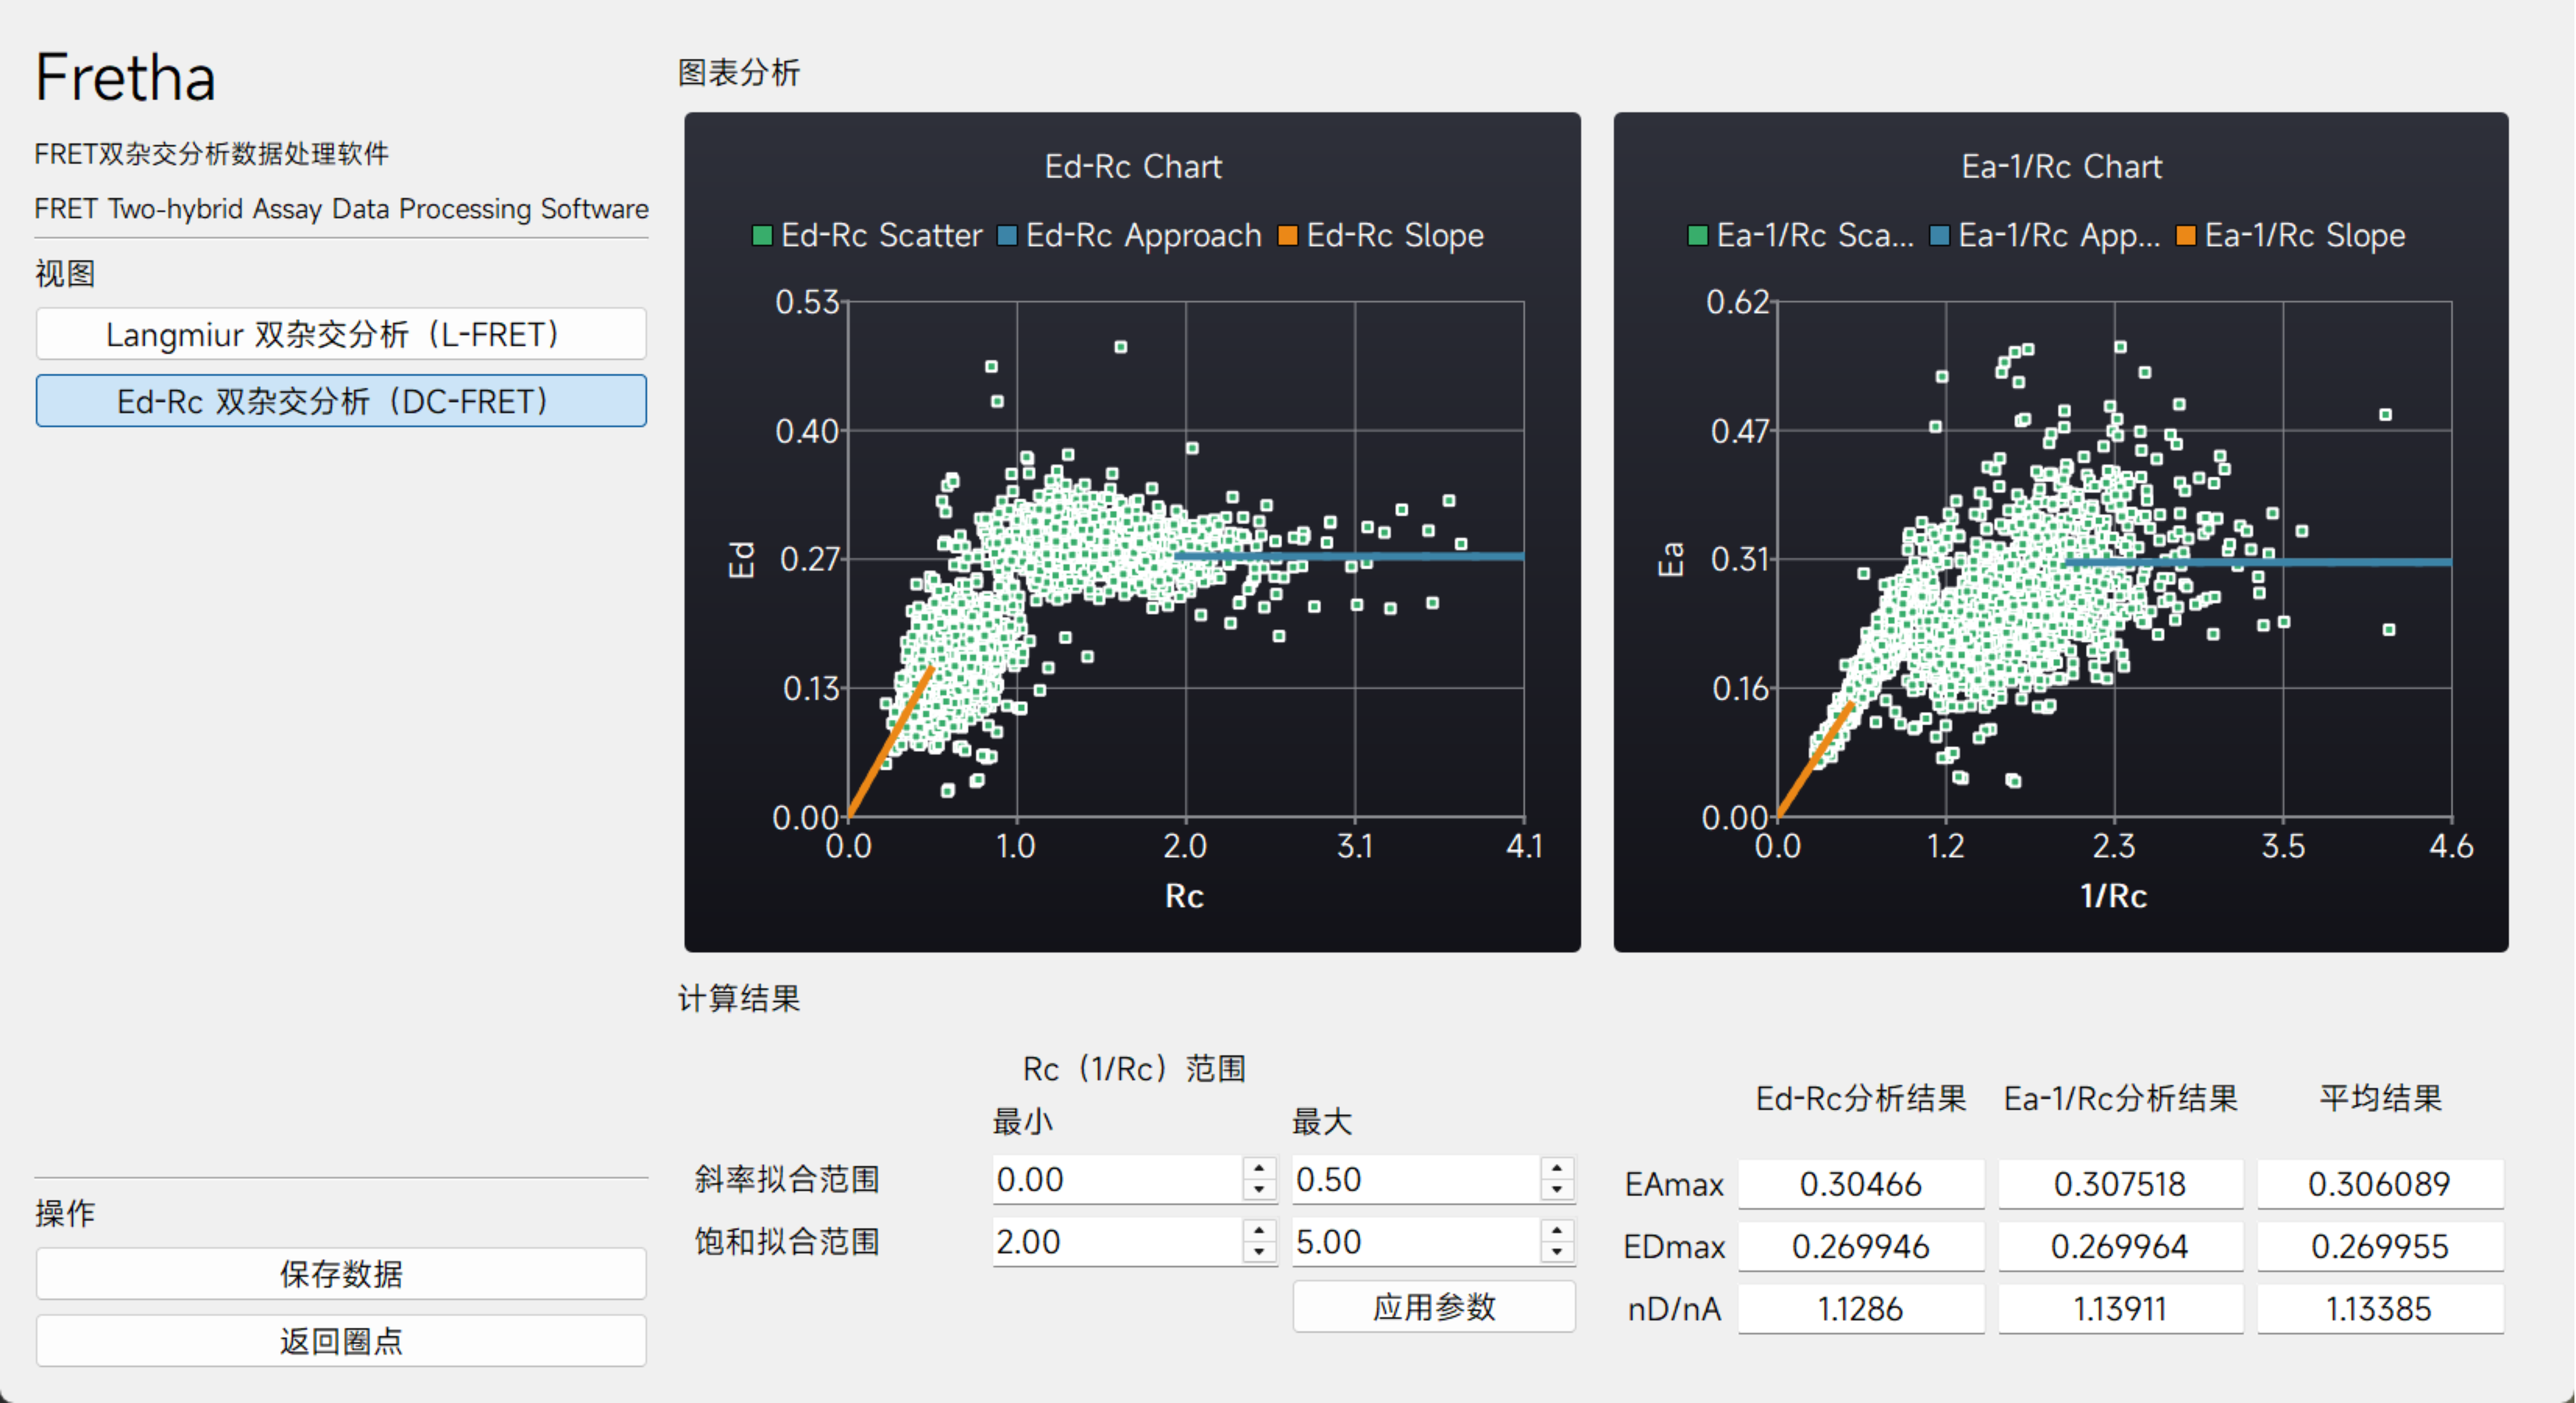
\includegraphics[width=0.9\linewidth]{../figures/2/2_DC-FRET结果界面.png}
  \caption{Fretha DC-FRET视图}
  \label{fig:fretha_dc_fret}
\end{figure}

DC-FRET视图的界面如图 \ref{fig:fretha_dc_fret} 所示。
在DC-FRET视图模式下,软件能显示出DC-FRET的拟合结果,包括$E_{A,max}$、$E_{D,max}$、$n_D/n_A$,以及拟合曲线和实验数据的对比图。
界面中设计了调整线性拟合参数的设置栏,用户可以调整$R_C$($1/R_C$)的数据范围,点击“更新”按钮以应用范围参数,用来处理复杂的数据。

点击“保存结果”按钮后,系统将同步存储拟合结果数据、可视化图像及实验数据,保存结果如图表所示。
\begin{table}[htbp]
  \centering
  \caption{结果保存生成文件}
  \label{tab:fretha_result_list}
    \begin{tabular}{cc}
      \toprule
      {文件名} & {说明} \\
      \hline
      Ea-Rda图.png & $E_A$-$1/R_C$散点和趋势线图 \\
      Ed-Rad图.png & $E_D$-$R_C$散点和趋势线图 \\
      Ea-Dfree图.png & $E_A$-$D_{free}$散点和趋势线图 \\
      Ed-Afree图.png & $E_D$-$A_{free}$散点和趋势线图 \\
      FretThaData.csv & FRET双杂交分析结果数据 \\
      FretThaResults.csv & FRET双杂交分析结果拟合参数 \\
      \bottomrule
    \end{tabular}
\end{table}
其中,实验数据与拟合参数的原始数值将以 CSV 文件格式进行保存,该文件包含可直接用于其他科研绘图软件的数据记录,从而支持用户在不同可视化工具中进行后续的图形优化与再处理。
这一功能设计保障了实验结果的完整留存,为科研工作者提供了灵活的数据导出与再分析解决方案。
\fi

\section{本章小结}

\ifshowtext
本章介绍了FRET双杂交分析数据处理软件(Fretha)的设计和开发。
Fretha采用分层架构设计,被分为表示层、业务层、数据访问层和数据层,从设计上尽可能地进行解耦,减少了冗余设计。
基于FRET双杂交分析数据处理的需求,Fretha在功能逻辑上划分为成像参数设置模块、数据校验模块、FRET图像处理模块、数据管理模块和结果可视化模块,然后通过分层架构完成了每个功能模块的开发。
得益于分层架构设计和功能模块化设计,Fretha实现了各种复杂数据处理功能,是一款拥有用户友好界面、简单易用、处理高效的科研数据处理软件。
\fi